\documentclass[twoside]{book}

% Packages required by doxygen
\usepackage{fixltx2e}
\usepackage{calc}
\usepackage{doxygen}
\usepackage[export]{adjustbox} % also loads graphicx
\usepackage{graphicx}
\usepackage[utf8]{inputenc}
\usepackage{makeidx}
\usepackage{multicol}
\usepackage{multirow}
\PassOptionsToPackage{warn}{textcomp}
\usepackage{textcomp}
\usepackage[nointegrals]{wasysym}
\usepackage[table]{xcolor}

% Font selection
\usepackage[T1]{fontenc}
\usepackage[scaled=.90]{helvet}
\usepackage{courier}
\usepackage{amssymb}
\usepackage{sectsty}
\renewcommand{\familydefault}{\sfdefault}
\allsectionsfont{%
  \fontseries{bc}\selectfont%
  \color{darkgray}%
}
\renewcommand{\DoxyLabelFont}{%
  \fontseries{bc}\selectfont%
  \color{darkgray}%
}
\newcommand{\+}{\discretionary{\mbox{\scriptsize$\hookleftarrow$}}{}{}}

% Page & text layout
\usepackage{geometry}
\geometry{%
  a4paper,%
  top=2.5cm,%
  bottom=2.5cm,%
  left=2.5cm,%
  right=2.5cm%
}
\tolerance=750
\hfuzz=15pt
\hbadness=750
\setlength{\emergencystretch}{15pt}
\setlength{\parindent}{0cm}
\setlength{\parskip}{0.2cm}
\makeatletter
\renewcommand{\paragraph}{%
  \@startsection{paragraph}{4}{0ex}{-1.0ex}{1.0ex}{%
    \normalfont\normalsize\bfseries\SS@parafont%
  }%
}
\renewcommand{\subparagraph}{%
  \@startsection{subparagraph}{5}{0ex}{-1.0ex}{1.0ex}{%
    \normalfont\normalsize\bfseries\SS@subparafont%
  }%
}
\makeatother

% Headers & footers
\usepackage{fancyhdr}
\pagestyle{fancyplain}
\fancyhead[LE]{\fancyplain{}{\bfseries\thepage}}
\fancyhead[CE]{\fancyplain{}{}}
\fancyhead[RE]{\fancyplain{}{\bfseries\leftmark}}
\fancyhead[LO]{\fancyplain{}{\bfseries\rightmark}}
\fancyhead[CO]{\fancyplain{}{}}
\fancyhead[RO]{\fancyplain{}{\bfseries\thepage}}
\fancyfoot[LE]{\fancyplain{}{}}
\fancyfoot[CE]{\fancyplain{}{}}
\fancyfoot[RE]{\fancyplain{}{\bfseries\scriptsize Generated on Tue Apr 14 2015 16\+:08\+:07 for Breakout by Doxygen }}
\fancyfoot[LO]{\fancyplain{}{\bfseries\scriptsize Generated on Tue Apr 14 2015 16\+:08\+:07 for Breakout by Doxygen }}
\fancyfoot[CO]{\fancyplain{}{}}
\fancyfoot[RO]{\fancyplain{}{}}
\renewcommand{\footrulewidth}{0.4pt}
\renewcommand{\chaptermark}[1]{%
  \markboth{#1}{}%
}
\renewcommand{\sectionmark}[1]{%
  \markright{\thesection\ #1}%
}

% Indices & bibliography
\usepackage{natbib}
\usepackage[titles]{tocloft}
\setcounter{tocdepth}{3}
\setcounter{secnumdepth}{5}
\makeindex

% Hyperlinks (required, but should be loaded last)
\usepackage{ifpdf}
\ifpdf
  \usepackage[pdftex,pagebackref=true]{hyperref}
\else
  \usepackage[ps2pdf,pagebackref=true]{hyperref}
\fi
\hypersetup{%
  colorlinks=true,%
  linkcolor=blue,%
  citecolor=blue,%
  unicode%
}

% Custom commands
\newcommand{\clearemptydoublepage}{%
  \newpage{\pagestyle{empty}\cleardoublepage}%
}


%===== C O N T E N T S =====

\begin{document}

% Titlepage & ToC
\hypersetup{pageanchor=false,
             bookmarks=true,
             bookmarksnumbered=true,
             pdfencoding=unicode
            }
\pagenumbering{roman}
\begin{titlepage}
\vspace*{7cm}
\begin{center}%
{\Large Breakout \\[1ex]\large 1.\+0 }\\
\vspace*{1cm}
{\large Generated by Doxygen 1.8.9.1}\\
\vspace*{0.5cm}
{\small Tue Apr 14 2015 16:08:07}\\
\end{center}
\end{titlepage}
\clearemptydoublepage
\tableofcontents
\clearemptydoublepage
\pagenumbering{arabic}
\hypersetup{pageanchor=true}

%--- Begin generated contents ---
\chapter{Hierarchical Index}
\section{Class Hierarchy}
This inheritance list is sorted roughly, but not completely, alphabetically\+:\begin{DoxyCompactList}
\item \contentsline{section}{Brick\+Factory}{\pageref{class_brick_factory}}{}
\item \contentsline{section}{Brick\+Fly\+Weight}{\pageref{class_brick_fly_weight}}{}
\item \contentsline{section}{Collision}{\pageref{class_collision}}{}
\item \contentsline{section}{Collision\+Manager}{\pageref{class_collision_manager}}{}
\item \contentsline{section}{Delta\+Timer}{\pageref{class_delta_timer}}{}
\item \contentsline{section}{File\+Handler}{\pageref{class_file_handler}}{}
\item \contentsline{section}{Game\+Manager}{\pageref{class_game_manager}}{}
\item \contentsline{section}{Game\+Object}{\pageref{class_game_object}}{}
\begin{DoxyCompactList}
\item \contentsline{section}{Ball}{\pageref{class_ball}}{}
\item \contentsline{section}{Brick}{\pageref{class_brick}}{}
\item \contentsline{section}{Player}{\pageref{class_player}}{}
\end{DoxyCompactList}
\item \contentsline{section}{Game\+Object\+Spawner$<$ T $>$}{\pageref{class_game_object_spawner}}{}
\item \contentsline{section}{Game\+Object\+Spawner$<$ Ball $>$}{\pageref{class_game_object_spawner}}{}
\item \contentsline{section}{Game\+Object\+Spawner$<$ Player $>$}{\pageref{class_game_object_spawner}}{}
\item \contentsline{section}{Input\+Manager}{\pageref{class_input_manager}}{}
\item \contentsline{section}{Level\+Manager}{\pageref{class_level_manager}}{}
\item runtime\+\_\+error\begin{DoxyCompactList}
\item \contentsline{section}{S\+D\+L\+Initialization\+Exception}{\pageref{class_s_d_l_initialization_exception}}{}
\end{DoxyCompactList}
\item \contentsline{section}{Score\+Manager}{\pageref{class_score_manager}}{}
\item \contentsline{section}{S\+D\+Lsound}{\pageref{class_s_d_lsound}}{}
\item \contentsline{section}{S\+D\+Lvideo}{\pageref{class_s_d_lvideo}}{}
\item \contentsline{section}{Updateable}{\pageref{class_updateable}}{}
\begin{DoxyCompactList}
\item \contentsline{section}{Component}{\pageref{class_component}}{}
\begin{DoxyCompactList}
\item \contentsline{section}{Collision\+Component}{\pageref{class_collision_component}}{}
\begin{DoxyCompactList}
\item \contentsline{section}{Ball\+Collision\+Component}{\pageref{class_ball_collision_component}}{}
\item \contentsline{section}{Brick\+Collision\+Component}{\pageref{class_brick_collision_component}}{}
\item \contentsline{section}{Player\+Collision\+Component}{\pageref{class_player_collision_component}}{}
\end{DoxyCompactList}
\item \contentsline{section}{Movement\+Component}{\pageref{class_movement_component}}{}
\begin{DoxyCompactList}
\item \contentsline{section}{Ball\+Movement\+Component}{\pageref{class_ball_movement_component}}{}
\item \contentsline{section}{Player\+Movement\+Component}{\pageref{class_player_movement_component}}{}
\end{DoxyCompactList}
\end{DoxyCompactList}
\end{DoxyCompactList}
\end{DoxyCompactList}

\chapter{Class Index}
\section{Class List}
Here are the classes, structs, unions and interfaces with brief descriptions\+:\begin{DoxyCompactList}
\item\contentsline{section}{\hyperlink{class_ball}{Ball} \\*This header file declares \hyperlink{class_ball}{Ball} subclass of \hyperlink{class_game_object}{Game\+Object} }{\pageref{class_ball}}{}
\item\contentsline{section}{\hyperlink{class_ball_collision_component}{Ball\+Collision\+Component} \\*This header file declares the component used for handling collisions in the \hyperlink{class_ball}{Ball} \hyperlink{class_game_object}{Game\+Object} }{\pageref{class_ball_collision_component}}{}
\item\contentsline{section}{\hyperlink{class_ball_movement_component}{Ball\+Movement\+Component} \\*This header file declares the component used for handling movement in the \hyperlink{class_ball}{Ball} \hyperlink{class_game_object}{Game\+Object} }{\pageref{class_ball_movement_component}}{}
\item\contentsline{section}{\hyperlink{class_brick}{Brick} \\*This header file declares the \hyperlink{class_brick}{Brick} subclass of \hyperlink{class_game_object}{Game\+Object} }{\pageref{class_brick}}{}
\item\contentsline{section}{\hyperlink{class_brick_collision_component}{Brick\+Collision\+Component} \\*This header file declares the component used for handling collisions in the \hyperlink{class_brick}{Brick} \hyperlink{class_game_object}{Game\+Object} }{\pageref{class_brick_collision_component}}{}
\item\contentsline{section}{\hyperlink{class_brick_factory}{Brick\+Factory} \\*Standard factory pattern for producing bricks with flyweights, tightly coupled with \hyperlink{class_level_manager}{Level\+Manager} and \hyperlink{class_s_d_lvideo}{S\+D\+Lvideo} for producing flyweight textures }{\pageref{class_brick_factory}}{}
\item\contentsline{section}{\hyperlink{class_brick_fly_weight}{Brick\+Fly\+Weight} \\*This header file declares a simple flyweight for different coloured bricks }{\pageref{class_brick_fly_weight}}{}
\item\contentsline{section}{\hyperlink{class_collision}{Collision} \\*This header file declares the \hyperlink{class_collision}{Collision} V\+O }{\pageref{class_collision}}{}
\item\contentsline{section}{\hyperlink{class_collision_component}{Collision\+Component} }{\pageref{class_collision_component}}{}
\item\contentsline{section}{\hyperlink{class_collision_manager}{Collision\+Manager} \\*This header file declares the \hyperlink{class_collision_manager}{Collision\+Manager} for my game }{\pageref{class_collision_manager}}{}
\item\contentsline{section}{\hyperlink{class_component}{Component} }{\pageref{class_component}}{}
\item\contentsline{section}{\hyperlink{class_delta_timer}{Delta\+Timer} \\*This header file declares the \hyperlink{class_delta_timer}{Delta\+Timer} }{\pageref{class_delta_timer}}{}
\item\contentsline{section}{\hyperlink{class_file_handler}{File\+Handler} \\*This header file declares the \hyperlink{class_file_handler}{File\+Handler} }{\pageref{class_file_handler}}{}
\item\contentsline{section}{\hyperlink{class_game_manager}{Game\+Manager} \\*This header file declares the \hyperlink{class_game_manager}{Game\+Manager} }{\pageref{class_game_manager}}{}
\item\contentsline{section}{\hyperlink{class_game_object}{Game\+Object} \\*This header file declares the base class for all Game\+Objects }{\pageref{class_game_object}}{}
\item\contentsline{section}{\hyperlink{class_game_object_spawner}{Game\+Object\+Spawner$<$ T $>$} \\*This header file declares my generic \hyperlink{class_game_object}{Game\+Object} spawner }{\pageref{class_game_object_spawner}}{}
\item\contentsline{section}{\hyperlink{class_input_manager}{Input\+Manager} \\*This header file declares the \hyperlink{class_input_manager}{Input\+Manager} }{\pageref{class_input_manager}}{}
\item\contentsline{section}{\hyperlink{class_level_manager}{Level\+Manager} \\*This header file declares the \hyperlink{class_level_manager}{Level\+Manager} }{\pageref{class_level_manager}}{}
\item\contentsline{section}{\hyperlink{class_movement_component}{Movement\+Component} }{\pageref{class_movement_component}}{}
\item\contentsline{section}{\hyperlink{class_player}{Player} \\*This header file declares the \hyperlink{class_player}{Player} subclass of \hyperlink{class_game_object}{Game\+Object} }{\pageref{class_player}}{}
\item\contentsline{section}{\hyperlink{class_player_collision_component}{Player\+Collision\+Component} \\*This header file declares the component used for handling collisions in the \hyperlink{class_player}{Player} \hyperlink{class_game_object}{Game\+Object} }{\pageref{class_player_collision_component}}{}
\item\contentsline{section}{\hyperlink{class_player_movement_component}{Player\+Movement\+Component} \\*This header file declares the component used for handling movement in the \hyperlink{class_player}{Player} \hyperlink{class_game_object}{Game\+Object} }{\pageref{class_player_movement_component}}{}
\item\contentsline{section}{\hyperlink{class_score_manager}{Score\+Manager} \\*This header file declares the \hyperlink{class_score_manager}{Score\+Manager} }{\pageref{class_score_manager}}{}
\item\contentsline{section}{\hyperlink{class_s_d_l_initialization_exception}{S\+D\+L\+Initialization\+Exception} \\*This header file declares the Exception class i made for showing that i understand how they work }{\pageref{class_s_d_l_initialization_exception}}{}
\item\contentsline{section}{\hyperlink{class_s_d_lsound}{S\+D\+Lsound} \\*This header file declares the facade for S\+D\+L\+\_\+mixer }{\pageref{class_s_d_lsound}}{}
\item\contentsline{section}{\hyperlink{class_s_d_lvideo}{S\+D\+Lvideo} \\*This header file declares the facade for S\+D\+L video rendering }{\pageref{class_s_d_lvideo}}{}
\item\contentsline{section}{\hyperlink{class_updateable}{Updateable} \\*This header file declares the different abstract and concrete interfaces I use for components }{\pageref{class_updateable}}{}
\end{DoxyCompactList}

\chapter{Class Documentation}
\hypertarget{class_ball}{}\section{Ball Class Reference}
\label{class_ball}\index{Ball@{Ball}}


This header file declares \hyperlink{class_ball}{Ball} subclass of \hyperlink{class_game_object}{Game\+Object}.  




{\ttfamily \#include $<$Ball.\+h$>$}

Inheritance diagram for Ball\+:\begin{figure}[H]
\begin{center}
\leavevmode
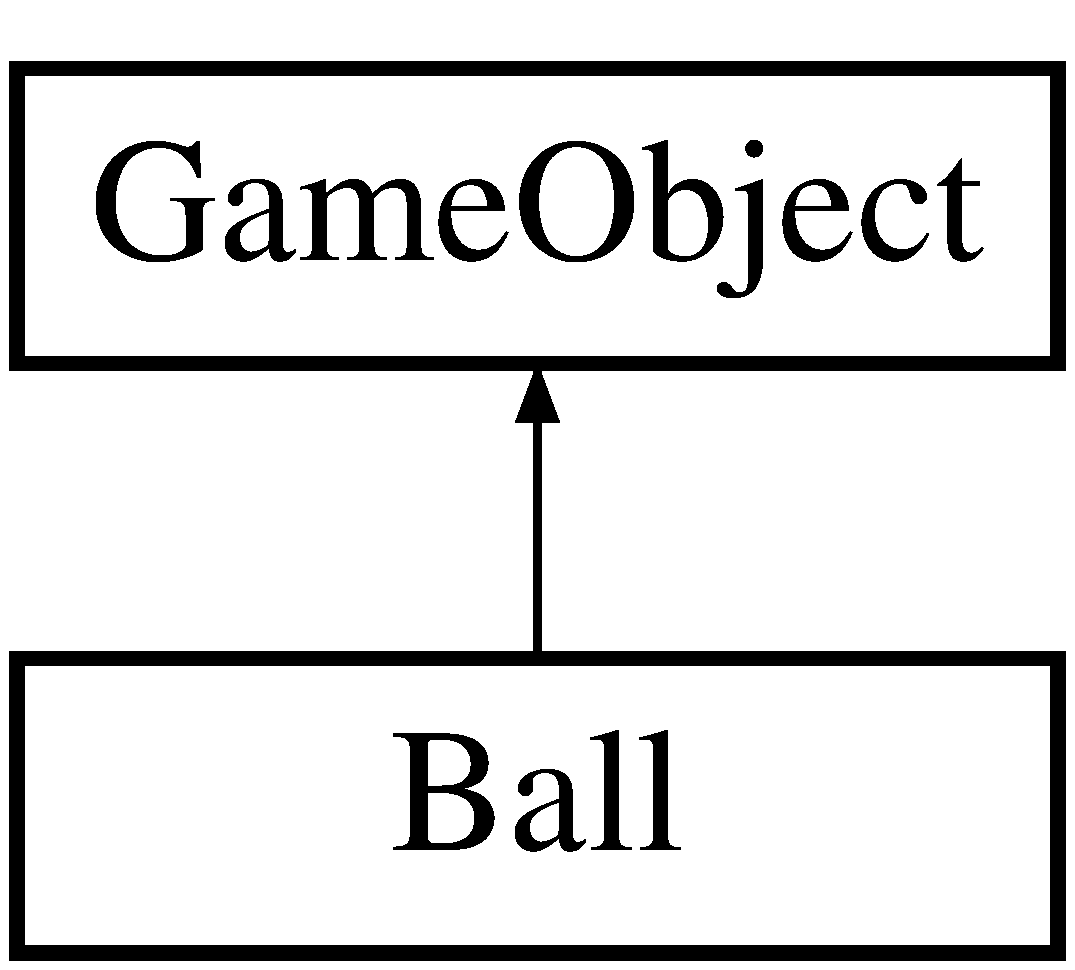
\includegraphics[height=2.000000cm]{class_ball}
\end{center}
\end{figure}
\subsection*{Public Member Functions}
\begin{DoxyCompactItemize}
\item 
\hypertarget{class_ball_acffa9c6b9fed01b0c9cd06cec8149a31}{}S\+D\+L\+\_\+\+Surface $\ast$ {\bfseries Get\+Surface} () const \label{class_ball_acffa9c6b9fed01b0c9cd06cec8149a31}

\item 
\hypertarget{class_ball_a883c0f3662079b64a825aa4f93306fb6}{}void {\bfseries Initialize\+Ball} ()\label{class_ball_a883c0f3662079b64a825aa4f93306fb6}

\item 
\hypertarget{class_ball_a206e7dbf1267fe178ba7ecabe705cff7}{}void {\bfseries Activate\+Ball} ()\label{class_ball_a206e7dbf1267fe178ba7ecabe705cff7}

\end{DoxyCompactItemize}
\subsection*{Friends}
\begin{DoxyCompactItemize}
\item 
\hypertarget{class_ball_aa58cdd45353dab2fd0d8e0da60621f73}{}class {\bfseries Ball\+Movement\+Component}\label{class_ball_aa58cdd45353dab2fd0d8e0da60621f73}

\item 
\hypertarget{class_ball_ad6767ce4b36efc15b7aae3cfde953c69}{}class {\bfseries Ball\+Collision\+Component}\label{class_ball_ad6767ce4b36efc15b7aae3cfde953c69}

\end{DoxyCompactItemize}
\subsection*{Additional Inherited Members}


\subsection{Detailed Description}
This header file declares \hyperlink{class_ball}{Ball} subclass of \hyperlink{class_game_object}{Game\+Object}. 

\begin{DoxyAuthor}{Author}
Anders Mikkelsen 
\end{DoxyAuthor}
\begin{DoxyVersion}{Version}
1.\+0 
\end{DoxyVersion}
\begin{DoxyDate}{Date}
13.\+04.\+2015 
\end{DoxyDate}


The documentation for this class was generated from the following files\+:\begin{DoxyCompactItemize}
\item 
Ball.\+h\item 
Ball.\+cpp\end{DoxyCompactItemize}

\hypertarget{class_ball_collision_component}{}\section{Ball\+Collision\+Component Class Reference}
\label{class_ball_collision_component}\index{Ball\+Collision\+Component@{Ball\+Collision\+Component}}


This header file declares the component used for handling collisions in the \hyperlink{class_ball}{Ball} \hyperlink{class_game_object}{Game\+Object}.  




{\ttfamily \#include $<$Ball\+Collision\+Component.\+h$>$}

Inheritance diagram for Ball\+Collision\+Component\+:\begin{figure}[H]
\begin{center}
\leavevmode
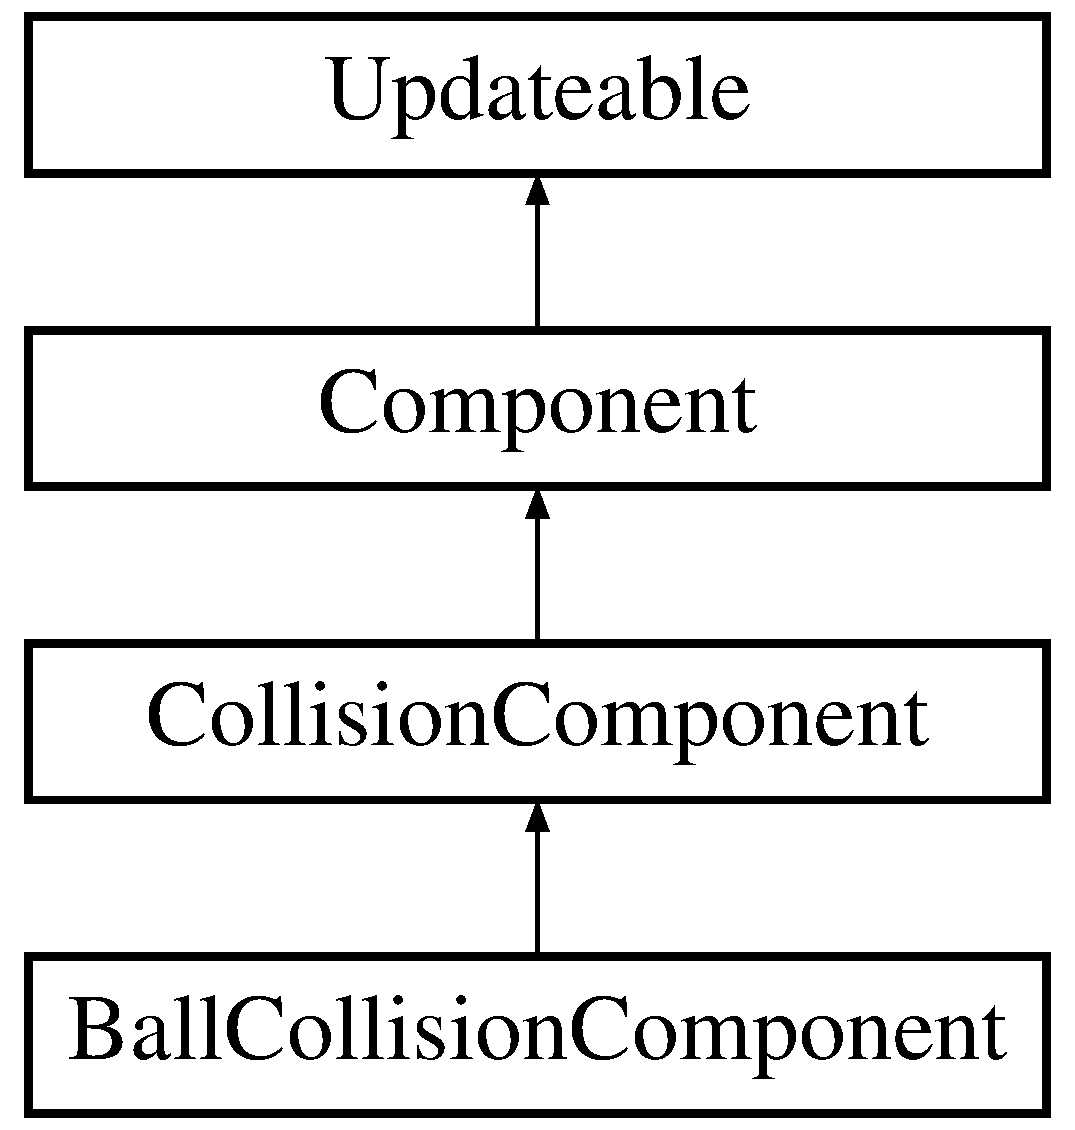
\includegraphics[height=4.000000cm]{class_ball_collision_component}
\end{center}
\end{figure}
\subsection*{Public Member Functions}
\begin{DoxyCompactItemize}
\item 
\hypertarget{class_ball_collision_component_a89716dc3b14195064f1ba82c1b59f5bb}{}{\bfseries Ball\+Collision\+Component} (\hyperlink{class_game_object}{Game\+Object} $\ast$const go)\label{class_ball_collision_component_a89716dc3b14195064f1ba82c1b59f5bb}

\item 
\hypertarget{class_ball_collision_component_a39e998b01d44fedb05e908a6f10e7202}{}void {\bfseries Update} () override\label{class_ball_collision_component_a39e998b01d44fedb05e908a6f10e7202}

\item 
\hypertarget{class_ball_collision_component_a51ce8485efacd4da61692b79a7d9a87c}{}void {\bfseries Handle\+Collision} (const \hyperlink{class_game_object}{Game\+Object} \&collidee) override\label{class_ball_collision_component_a51ce8485efacd4da61692b79a7d9a87c}

\end{DoxyCompactItemize}
\subsection*{Protected Member Functions}
\begin{DoxyCompactItemize}
\item 
\hypertarget{class_ball_collision_component_a9837dc881118a8301c12fe3e84eef29c}{}void {\bfseries Handle\+Player\+Collision} (const \hyperlink{class_player}{Player} \&collidee)\label{class_ball_collision_component_a9837dc881118a8301c12fe3e84eef29c}

\item 
\hypertarget{class_ball_collision_component_a1f582b16fc10e8c23245ce6a204c316d}{}void {\bfseries Handle\+Brick\+Collision} (const \hyperlink{class_brick}{Brick} \&collidee)\label{class_ball_collision_component_a1f582b16fc10e8c23245ce6a204c316d}

\item 
\hypertarget{class_ball_collision_component_a609fe70bf85ba2c9b28d2812cc036892}{}bool {\bfseries Check\+For\+Wall\+Collision} ()\label{class_ball_collision_component_a609fe70bf85ba2c9b28d2812cc036892}

\end{DoxyCompactItemize}
\subsection*{Protected Attributes}
\begin{DoxyCompactItemize}
\item 
\hypertarget{class_ball_collision_component_a0dbf72b26b0ee1311f94fb3aae543f98}{}\hyperlink{class_ball}{Ball} $\ast$ {\bfseries ball\+\_\+}\label{class_ball_collision_component_a0dbf72b26b0ee1311f94fb3aae543f98}

\end{DoxyCompactItemize}


\subsection{Detailed Description}
This header file declares the component used for handling collisions in the \hyperlink{class_ball}{Ball} \hyperlink{class_game_object}{Game\+Object}. 

It is updated every frame and is called by Handle\+Collision if involved in a collision.

\begin{DoxyAuthor}{Author}
Anders Mikkelsen 
\end{DoxyAuthor}
\begin{DoxyVersion}{Version}
1.\+0 
\end{DoxyVersion}
\begin{DoxyDate}{Date}
13.\+04.\+2015 
\end{DoxyDate}


The documentation for this class was generated from the following files\+:\begin{DoxyCompactItemize}
\item 
Ball\+Collision\+Component.\+h\item 
Ball\+Collision\+Component.\+cpp\end{DoxyCompactItemize}

\hypertarget{class_ball_movement_component}{}\section{Ball\+Movement\+Component Class Reference}
\label{class_ball_movement_component}\index{Ball\+Movement\+Component@{Ball\+Movement\+Component}}


This header file declares the component used for handling movement in the \hyperlink{class_ball}{Ball} \hyperlink{class_game_object}{Game\+Object}.  




{\ttfamily \#include $<$Ball\+Movement\+Component.\+h$>$}

Inheritance diagram for Ball\+Movement\+Component\+:\begin{figure}[H]
\begin{center}
\leavevmode
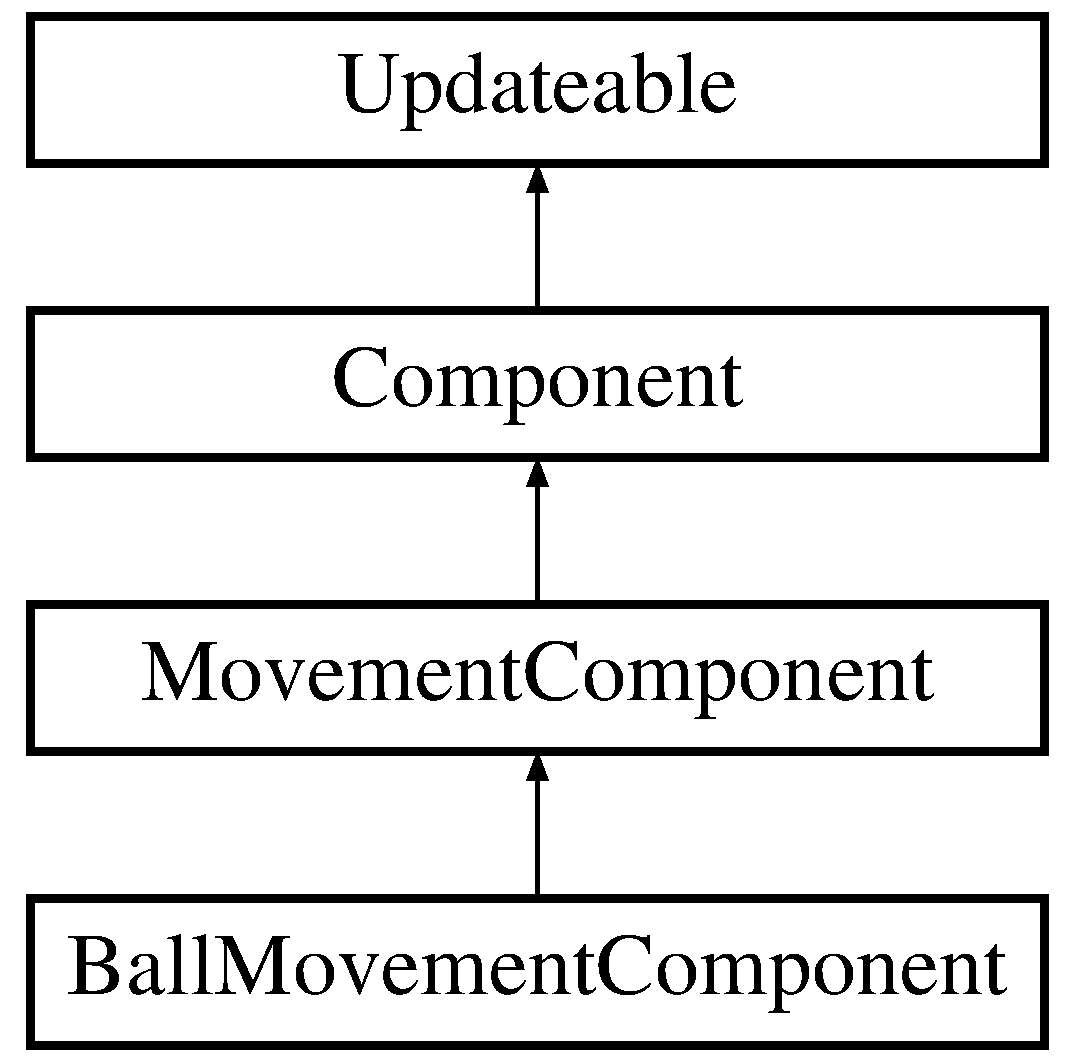
\includegraphics[height=4.000000cm]{class_ball_movement_component}
\end{center}
\end{figure}
\subsection*{Public Member Functions}
\begin{DoxyCompactItemize}
\item 
\hypertarget{class_ball_movement_component_a49bff8098e0187712b8b0e176606c5b7}{}{\bfseries Ball\+Movement\+Component} (\hyperlink{class_game_object}{Game\+Object} $\ast$const go)\label{class_ball_movement_component_a49bff8098e0187712b8b0e176606c5b7}

\item 
\hypertarget{class_ball_movement_component_ab538dd44c8dd7cd0fc606bb579a67c71}{}void {\bfseries Update} () override\label{class_ball_movement_component_ab538dd44c8dd7cd0fc606bb579a67c71}

\end{DoxyCompactItemize}
\subsection*{Additional Inherited Members}


\subsection{Detailed Description}
This header file declares the component used for handling movement in the \hyperlink{class_ball}{Ball} \hyperlink{class_game_object}{Game\+Object}. 

It is updated every frame.

\begin{DoxyAuthor}{Author}
Anders Mikkelsen 
\end{DoxyAuthor}
\begin{DoxyVersion}{Version}
1.\+0 
\end{DoxyVersion}
\begin{DoxyDate}{Date}
13.\+04.\+2015 
\end{DoxyDate}


The documentation for this class was generated from the following files\+:\begin{DoxyCompactItemize}
\item 
Ball\+Movement\+Component.\+h\item 
Ball\+Movement\+Component.\+cpp\end{DoxyCompactItemize}

\hypertarget{class_brick}{}\section{Brick Class Reference}
\label{class_brick}\index{Brick@{Brick}}


This header file declares the \hyperlink{class_brick}{Brick} subclass of \hyperlink{class_game_object}{Game\+Object}.  




{\ttfamily \#include $<$Brick.\+h$>$}

Inheritance diagram for Brick\+:\begin{figure}[H]
\begin{center}
\leavevmode
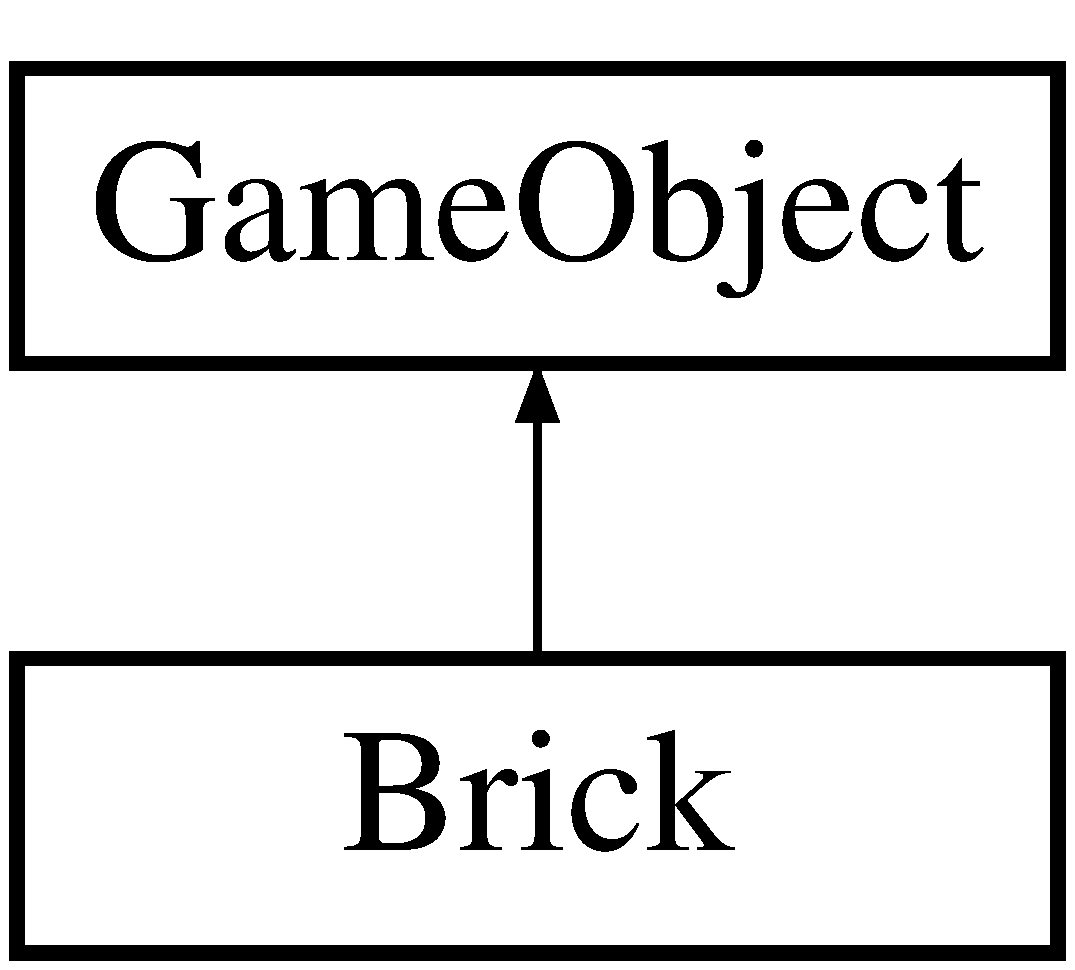
\includegraphics[height=2.000000cm]{class_brick}
\end{center}
\end{figure}
\subsection*{Public Member Functions}
\begin{DoxyCompactItemize}
\item 
\hypertarget{class_brick_af7fc5d103be6a189107ad348b097c79d}{}{\bfseries Brick} (\hyperlink{class_brick_fly_weight}{Brick\+Fly\+Weight} brick\+\_\+fly\+\_\+weight\+\_\+)\label{class_brick_af7fc5d103be6a189107ad348b097c79d}

\item 
\hypertarget{class_brick_a491c5e8532641813149eaba714dc067d}{}const \hyperlink{class_brick_fly_weight}{Brick\+Fly\+Weight} $\ast$ {\bfseries Get\+Brick\+Fly\+Weight} () const \label{class_brick_a491c5e8532641813149eaba714dc067d}

\end{DoxyCompactItemize}
\subsection*{Friends}
\begin{DoxyCompactItemize}
\item 
\hypertarget{class_brick_abbe1e4d04c25e93f121c0b0b0bba6dbd}{}class {\bfseries Brick\+Collision\+Component}\label{class_brick_abbe1e4d04c25e93f121c0b0b0bba6dbd}

\end{DoxyCompactItemize}
\subsection*{Additional Inherited Members}


\subsection{Detailed Description}
This header file declares the \hyperlink{class_brick}{Brick} subclass of \hyperlink{class_game_object}{Game\+Object}. 

\begin{DoxyAuthor}{Author}
Anders Mikkelsen 
\end{DoxyAuthor}
\begin{DoxyVersion}{Version}
1.\+0 
\end{DoxyVersion}
\begin{DoxyDate}{Date}
13.\+04.\+2015 
\end{DoxyDate}


The documentation for this class was generated from the following files\+:\begin{DoxyCompactItemize}
\item 
Brick.\+h\item 
Brick.\+cpp\end{DoxyCompactItemize}

\hypertarget{class_brick_collision_component}{}\section{Brick\+Collision\+Component Class Reference}
\label{class_brick_collision_component}\index{Brick\+Collision\+Component@{Brick\+Collision\+Component}}


This header file declares the component used for handling collisions in the \hyperlink{class_brick}{Brick} \hyperlink{class_game_object}{Game\+Object}.  




{\ttfamily \#include $<$Brick\+Collision\+Component.\+h$>$}

Inheritance diagram for Brick\+Collision\+Component\+:\begin{figure}[H]
\begin{center}
\leavevmode
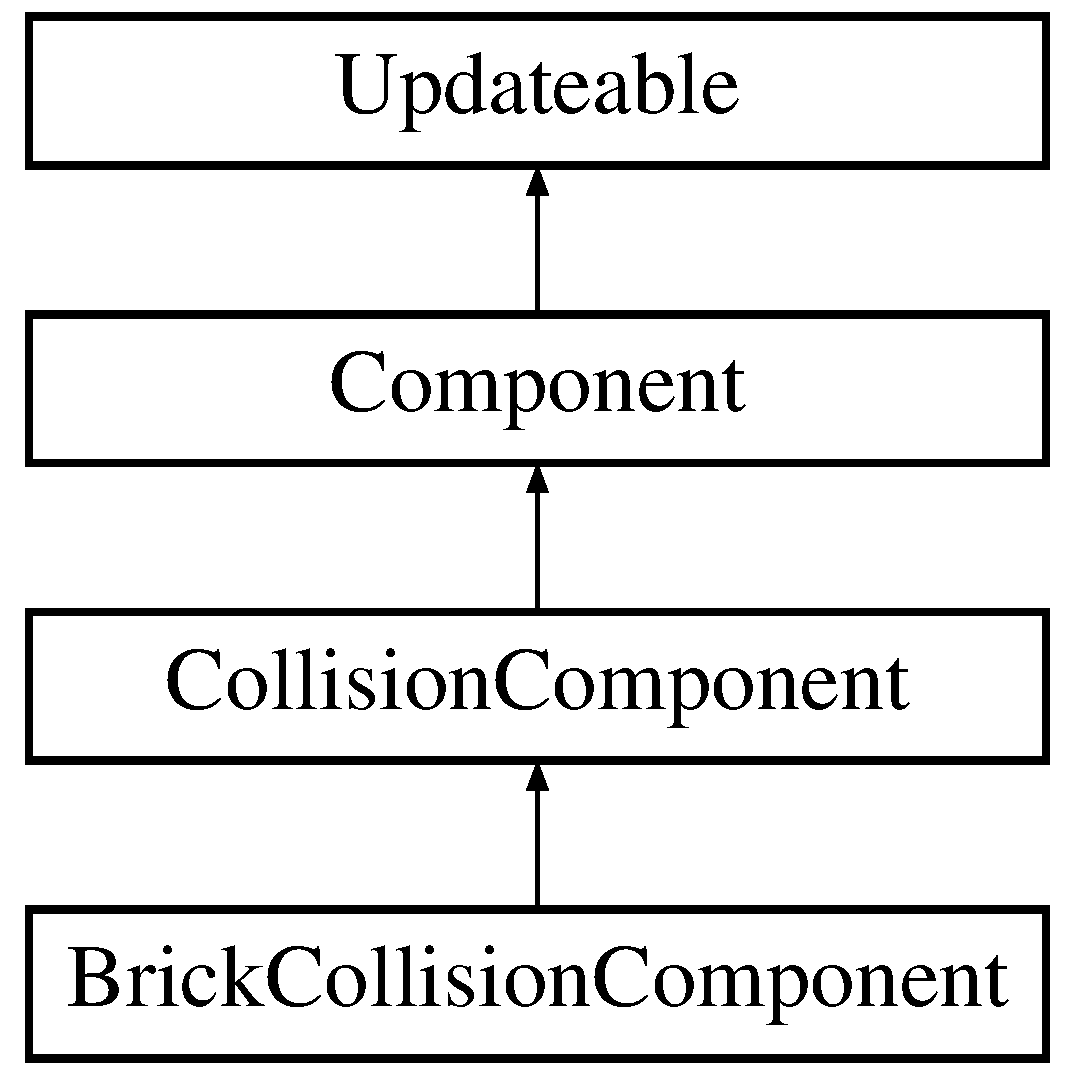
\includegraphics[height=4.000000cm]{class_brick_collision_component}
\end{center}
\end{figure}
\subsection*{Public Member Functions}
\begin{DoxyCompactItemize}
\item 
\hypertarget{class_brick_collision_component_ac2c7dfafc9fea0857d018e52879a9847}{}{\bfseries Brick\+Collision\+Component} (\hyperlink{class_game_object}{Game\+Object} $\ast$const go)\label{class_brick_collision_component_ac2c7dfafc9fea0857d018e52879a9847}

\item 
\hypertarget{class_brick_collision_component_a944b2ff38843cda6bd387a198470552c}{}void {\bfseries Update} () override\label{class_brick_collision_component_a944b2ff38843cda6bd387a198470552c}

\item 
\hypertarget{class_brick_collision_component_a601bd53d0b9e8383e6a5e47d549587ab}{}void {\bfseries Handle\+Collision} (const \hyperlink{class_game_object}{Game\+Object} \&collidee) override\label{class_brick_collision_component_a601bd53d0b9e8383e6a5e47d549587ab}

\end{DoxyCompactItemize}
\subsection*{Protected Attributes}
\begin{DoxyCompactItemize}
\item 
\hypertarget{class_brick_collision_component_af80c273547fd6e0e8046183dea6f3105}{}\hyperlink{class_brick}{Brick} $\ast$ {\bfseries brick\+\_\+}\label{class_brick_collision_component_af80c273547fd6e0e8046183dea6f3105}

\end{DoxyCompactItemize}


\subsection{Detailed Description}
This header file declares the component used for handling collisions in the \hyperlink{class_brick}{Brick} \hyperlink{class_game_object}{Game\+Object}. 

It is updated every frame and is called by Handle\+Collision if involved in a collision.

\begin{DoxyAuthor}{Author}
Anders Mikkelsen 
\end{DoxyAuthor}
\begin{DoxyVersion}{Version}
1.\+0 
\end{DoxyVersion}
\begin{DoxyDate}{Date}
13.\+04.\+2015 
\end{DoxyDate}


The documentation for this class was generated from the following files\+:\begin{DoxyCompactItemize}
\item 
Brick\+Collision\+Component.\+h\item 
Brick\+Collision\+Component.\+cpp\end{DoxyCompactItemize}

\hypertarget{class_brick_factory}{}\section{Brick\+Factory Class Reference}
\label{class_brick_factory}\index{Brick\+Factory@{Brick\+Factory}}


Standard factory pattern for producing bricks with flyweights, tightly coupled with \hyperlink{class_level_manager}{Level\+Manager} and \hyperlink{class_s_d_lvideo}{S\+D\+Lvideo} for producing flyweight textures.  




{\ttfamily \#include $<$Brick\+Factory.\+h$>$}

\subsection*{Public Types}
\begin{DoxyCompactItemize}
\item 
\hypertarget{class_brick_factory_a1b4958389153a74f1e6baf8ede9e000b}{}typedef std\+::shared\+\_\+ptr$<$ \hyperlink{class_brick}{Brick} $>$ {\bfseries shared\+\_\+ptr\+\_\+brick}\label{class_brick_factory_a1b4958389153a74f1e6baf8ede9e000b}

\end{DoxyCompactItemize}
\subsection*{Public Member Functions}
\begin{DoxyCompactItemize}
\item 
\hypertarget{class_brick_factory_a12dd1e3839193e381bc7198a876e472a}{}shared\+\_\+ptr\+\_\+brick {\bfseries Get\+Brick} (Brick\+Fly\+Weight\+::\+E\+Brick\+Type const brick\+\_\+type)\label{class_brick_factory_a12dd1e3839193e381bc7198a876e472a}

\item 
\hypertarget{class_brick_factory_a1dd70396dcdfc7ae2f5e1168b91d6bed}{}void {\bfseries Free\+All\+Surfaces} ()\label{class_brick_factory_a1dd70396dcdfc7ae2f5e1168b91d6bed}

\item 
\hypertarget{class_brick_factory_a200cfa3d335ed9291d6aa3e80227cb7d}{}void {\bfseries Clean\+Up} ()\label{class_brick_factory_a200cfa3d335ed9291d6aa3e80227cb7d}

\end{DoxyCompactItemize}


\subsection{Detailed Description}
Standard factory pattern for producing bricks with flyweights, tightly coupled with \hyperlink{class_level_manager}{Level\+Manager} and \hyperlink{class_s_d_lvideo}{S\+D\+Lvideo} for producing flyweight textures. 

\begin{DoxyAuthor}{Author}
Anders Mikkelsen 
\end{DoxyAuthor}
\begin{DoxyVersion}{Version}
1.\+0 
\end{DoxyVersion}
\begin{DoxyDate}{Date}
13.\+04.\+2015 
\end{DoxyDate}


The documentation for this class was generated from the following files\+:\begin{DoxyCompactItemize}
\item 
Brick\+Factory.\+h\item 
Brick\+Factory.\+cpp\end{DoxyCompactItemize}

\hypertarget{class_brick_fly_weight}{}\section{Brick\+Fly\+Weight Class Reference}
\label{class_brick_fly_weight}\index{Brick\+Fly\+Weight@{Brick\+Fly\+Weight}}


This header file declares a simple flyweight for different coloured bricks.  




{\ttfamily \#include $<$Brick\+Fly\+Weight.\+h$>$}

\subsection*{Public Types}
\begin{DoxyCompactItemize}
\item 
\hypertarget{class_brick_fly_weight_af4fde2a530a03e1ed036791793ceb4f0}{}enum {\bfseries E\+Brick\+Type} \{ \\*
{\bfseries R\+E\+D}, 
{\bfseries O\+R\+A\+N\+G\+E}, 
{\bfseries Y\+E\+L\+L\+O\+W}, 
{\bfseries B\+R\+O\+W\+N}, 
\\*
{\bfseries B\+L\+U\+E}, 
{\bfseries G\+R\+E\+E\+N}
 \}\label{class_brick_fly_weight_af4fde2a530a03e1ed036791793ceb4f0}

\end{DoxyCompactItemize}
\subsection*{Public Member Functions}
\begin{DoxyCompactItemize}
\item 
\hypertarget{class_brick_fly_weight_a7c287926919f47b3d554428d15c1fa25}{}{\bfseries Brick\+Fly\+Weight} (S\+D\+L\+\_\+\+Surface $\ast$const brick\+\_\+bmp, E\+Brick\+Type const brick\+\_\+type)\label{class_brick_fly_weight_a7c287926919f47b3d554428d15c1fa25}

\item 
\hypertarget{class_brick_fly_weight_ae8727465822b43dcecbff00538d9617a}{}const S\+D\+L\+\_\+\+Surface $\ast$ {\bfseries Get\+Brick\+Surface} () const \label{class_brick_fly_weight_ae8727465822b43dcecbff00538d9617a}

\item 
\hypertarget{class_brick_fly_weight_adf9c46301edbc8e78193fadc7f93895b}{}E\+Brick\+Type {\bfseries Get\+Brick\+Type} () const \label{class_brick_fly_weight_adf9c46301edbc8e78193fadc7f93895b}

\end{DoxyCompactItemize}


\subsection{Detailed Description}
This header file declares a simple flyweight for different coloured bricks. 

\begin{DoxyAuthor}{Author}
Anders Mikkelsen 
\end{DoxyAuthor}
\begin{DoxyVersion}{Version}
1.\+0 
\end{DoxyVersion}
\begin{DoxyDate}{Date}
13.\+04.\+2015 
\end{DoxyDate}


The documentation for this class was generated from the following files\+:\begin{DoxyCompactItemize}
\item 
Brick\+Fly\+Weight.\+h\item 
Brick\+Fly\+Weight.\+cpp\end{DoxyCompactItemize}

\hypertarget{class_collision}{}\section{Collision Class Reference}
\label{class_collision}\index{Collision@{Collision}}


This header file declares the \hyperlink{class_collision}{Collision} V\+O.  




{\ttfamily \#include $<$Collision.\+h$>$}

\subsection*{Public Member Functions}
\begin{DoxyCompactItemize}
\item 
\hypertarget{class_collision_a90b043fa38e90c4170c097191e91b9b2}{}{\bfseries Collision} (\hyperlink{class_game_object}{Game\+Object} const \&one, \hyperlink{class_game_object}{Game\+Object} const \&two)\label{class_collision_a90b043fa38e90c4170c097191e91b9b2}

\item 
\hypertarget{class_collision_adeb802af5ebc0abb67088ded28caf9ff}{}const \hyperlink{class_game_object}{Game\+Object} $\ast$ {\bfseries Get\+One} () const \label{class_collision_adeb802af5ebc0abb67088ded28caf9ff}

\item 
\hypertarget{class_collision_a6d3b7a8a023e7d26db89897f387dac7b}{}const \hyperlink{class_game_object}{Game\+Object} $\ast$ {\bfseries Get\+Two} () const \label{class_collision_a6d3b7a8a023e7d26db89897f387dac7b}

\end{DoxyCompactItemize}


\subsection{Detailed Description}
This header file declares the \hyperlink{class_collision}{Collision} V\+O. 

It holds a pointer to two \hyperlink{class_game_object}{Game\+Object}\textquotesingle{}s in a collision scenario.

\begin{DoxyAuthor}{Author}
Anders Mikkelsen 
\end{DoxyAuthor}
\begin{DoxyVersion}{Version}
1.\+0 
\end{DoxyVersion}
\begin{DoxyDate}{Date}
13.\+04.\+2015 
\end{DoxyDate}


The documentation for this class was generated from the following files\+:\begin{DoxyCompactItemize}
\item 
Collision.\+h\item 
Collision.\+cpp\end{DoxyCompactItemize}

\hypertarget{class_collision_component}{}\section{Collision\+Component Class Reference}
\label{class_collision_component}\index{Collision\+Component@{Collision\+Component}}
Inheritance diagram for Collision\+Component\+:\begin{figure}[H]
\begin{center}
\leavevmode
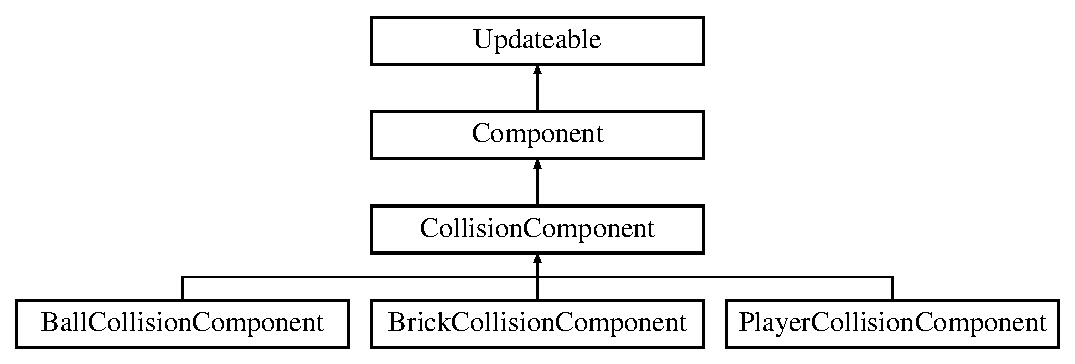
\includegraphics[height=4.000000cm]{class_collision_component}
\end{center}
\end{figure}
\subsection*{Public Member Functions}
\begin{DoxyCompactItemize}
\item 
\hypertarget{class_collision_component_a59f812bb26b98b655b822b667b07faf4}{}{\bfseries Collision\+Component} (\hyperlink{class_game_object}{Game\+Object} $\ast$const go)\label{class_collision_component_a59f812bb26b98b655b822b667b07faf4}

\item 
\hypertarget{class_collision_component_a182926fa0c68d147a06e510ef06c24e4}{}virtual void {\bfseries Update} () override\label{class_collision_component_a182926fa0c68d147a06e510ef06c24e4}

\item 
\hypertarget{class_collision_component_affd40acce224837439308535f329ccd9}{}virtual void {\bfseries Handle\+Collision} (const \hyperlink{class_game_object}{Game\+Object} \&)\label{class_collision_component_affd40acce224837439308535f329ccd9}

\end{DoxyCompactItemize}
\subsection*{Additional Inherited Members}


The documentation for this class was generated from the following file\+:\begin{DoxyCompactItemize}
\item 
Component.\+h\end{DoxyCompactItemize}

\hypertarget{class_collision_manager}{}\section{Collision\+Manager Class Reference}
\label{class_collision_manager}\index{Collision\+Manager@{Collision\+Manager}}


This header file declares the \hyperlink{class_collision_manager}{Collision\+Manager} for my game.  




{\ttfamily \#include $<$Collision\+Manager.\+h$>$}

\subsection*{Public Types}
\begin{DoxyCompactItemize}
\item 
\hypertarget{class_collision_manager_a41e4913345084ce048c9c8ad96bdeafe}{}typedef std\+::unique\+\_\+ptr$<$ std\+::vector$<$ std\+::shared\+\_\+ptr$<$ \hyperlink{class_collision}{Collision} $>$ $>$ $>$ {\bfseries vector\+\_\+of\+\_\+collisions}\label{class_collision_manager_a41e4913345084ce048c9c8ad96bdeafe}

\end{DoxyCompactItemize}
\subsection*{Public Member Functions}
\begin{DoxyCompactItemize}
\item 
\hypertarget{class_collision_manager_a8080db3a454be3b32505713bc6c3b1b3}{}void {\bfseries Add\+Game\+Object\+To\+Collision\+Grid} (\hyperlink{class_game_object}{Game\+Object} \&go)\label{class_collision_manager_a8080db3a454be3b32505713bc6c3b1b3}

\item 
\hypertarget{class_collision_manager_aa58022d2f80eb264c6f66e92a7209cf8}{}void {\bfseries Update\+Game\+Object\+Position} (\hyperlink{class_game_object}{Game\+Object} \&go)\label{class_collision_manager_aa58022d2f80eb264c6f66e92a7209cf8}

\item 
\hypertarget{class_collision_manager_ac1b05ae3761a90c75820edece9c7f938}{}void {\bfseries Remove\+Game\+Object\+From\+Collision\+Grid} (\hyperlink{class_game_object}{Game\+Object} \&go)\label{class_collision_manager_ac1b05ae3761a90c75820edece9c7f938}

\item 
\hypertarget{class_collision_manager_adb6ac040ca57dd43a1cff9e04ab3ab9d}{}vector\+\_\+of\+\_\+collisions {\bfseries Check\+For\+Collisions} (const \hyperlink{class_game_object}{Game\+Object} \&go)\label{class_collision_manager_adb6ac040ca57dd43a1cff9e04ab3ab9d}

\item 
\hypertarget{class_collision_manager_a3b1e3278a8aa71146b3cbb83e8f88d6b}{}void {\bfseries Clean\+Up} ()\label{class_collision_manager_a3b1e3278a8aa71146b3cbb83e8f88d6b}

\end{DoxyCompactItemize}


\subsection{Detailed Description}
This header file declares the \hyperlink{class_collision_manager}{Collision\+Manager} for my game. 

It uses a spatial partitioning grid and checks single objects against it. It\textquotesingle{}s is designed to only be sent movables every frame. That compared with a spatial partioning grid and a simple Bounding\+Box collision detection gives great performance!

\begin{DoxyAuthor}{Author}
Anders Mikkelsen 
\end{DoxyAuthor}
\begin{DoxyVersion}{Version}
1.\+0 
\end{DoxyVersion}
\begin{DoxyDate}{Date}
13.\+04.\+2015 
\end{DoxyDate}


The documentation for this class was generated from the following files\+:\begin{DoxyCompactItemize}
\item 
Collision\+Manager.\+h\item 
Collision\+Manager.\+cpp\end{DoxyCompactItemize}

\hypertarget{class_component}{}\section{Component Class Reference}
\label{class_component}\index{Component@{Component}}
Inheritance diagram for Component\+:\begin{figure}[H]
\begin{center}
\leavevmode
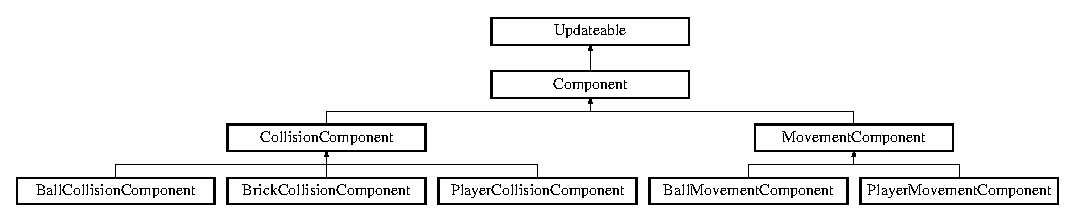
\includegraphics[height=2.516854cm]{class_component}
\end{center}
\end{figure}
\subsection*{Public Member Functions}
\begin{DoxyCompactItemize}
\item 
\hypertarget{class_component_aed6d43c7dda98b169f49e0485303d9f1}{}{\bfseries Component} (\hyperlink{class_game_object}{Game\+Object} $\ast$const go)\label{class_component_aed6d43c7dda98b169f49e0485303d9f1}

\item 
\hypertarget{class_component_a831c307a54d6ca9e5a75e2fc72770e63}{}\hyperlink{class_game_object}{Game\+Object} $\ast$ {\bfseries Get\+Owner} ()\label{class_component_a831c307a54d6ca9e5a75e2fc72770e63}

\end{DoxyCompactItemize}
\subsection*{Protected Attributes}
\begin{DoxyCompactItemize}
\item 
\hypertarget{class_component_a715fc40771d21d6d43d8209dd5c9810a}{}\hyperlink{class_game_object}{Game\+Object} $\ast$ {\bfseries owner}\label{class_component_a715fc40771d21d6d43d8209dd5c9810a}

\end{DoxyCompactItemize}


The documentation for this class was generated from the following file\+:\begin{DoxyCompactItemize}
\item 
Component.\+h\end{DoxyCompactItemize}

\hypertarget{class_delta_timer}{}\section{Delta\+Timer Class Reference}
\label{class_delta_timer}\index{Delta\+Timer@{Delta\+Timer}}


This header file declares the \hyperlink{class_delta_timer}{Delta\+Timer}.  




{\ttfamily \#include $<$Delta\+Timer.\+h$>$}

\subsection*{Public Member Functions}
\begin{DoxyCompactItemize}
\item 
\hypertarget{class_delta_timer_a6faf59a8023f9782941e36e18d00e7ea}{}void {\bfseries Start} ()\label{class_delta_timer_a6faf59a8023f9782941e36e18d00e7ea}

\item 
\hypertarget{class_delta_timer_a8a14b90c655e0ad93f17e951b5ea10d5}{}void {\bfseries Update} ()\label{class_delta_timer_a8a14b90c655e0ad93f17e951b5ea10d5}

\item 
\hypertarget{class_delta_timer_a0f9a9e94e8cfea5f16b7551049ca0e39}{}const float \& {\bfseries Get\+Delta\+Time} ()\label{class_delta_timer_a0f9a9e94e8cfea5f16b7551049ca0e39}

\item 
\hypertarget{class_delta_timer_a705657924511a8042e9dd7157bb617c9}{}void {\bfseries Pause} ()\label{class_delta_timer_a705657924511a8042e9dd7157bb617c9}

\item 
\hypertarget{class_delta_timer_a383c48dd4022656ed9c5affbcb71e9a1}{}void {\bfseries Un\+Pause} ()\label{class_delta_timer_a383c48dd4022656ed9c5affbcb71e9a1}

\item 
\hypertarget{class_delta_timer_aad80d6c4f6e52ffb46de3de3c61a5140}{}void {\bfseries Reset} ()\label{class_delta_timer_aad80d6c4f6e52ffb46de3de3c61a5140}

\end{DoxyCompactItemize}


\subsection{Detailed Description}
This header file declares the \hyperlink{class_delta_timer}{Delta\+Timer}. 

It is loosely based on the timer shown in class and the timer from Lazy Foo.

\begin{DoxyAuthor}{Author}
Anders Mikkelsen 
\end{DoxyAuthor}
\begin{DoxyVersion}{Version}
1.\+0 
\end{DoxyVersion}
\begin{DoxyDate}{Date}
13.\+04.\+2015 
\end{DoxyDate}


The documentation for this class was generated from the following files\+:\begin{DoxyCompactItemize}
\item 
Delta\+Timer.\+h\item 
Delta\+Timer.\+cpp\end{DoxyCompactItemize}

\hypertarget{class_file_handler}{}\section{File\+Handler Class Reference}
\label{class_file_handler}\index{File\+Handler@{File\+Handler}}


This header file declares the \hyperlink{class_file_handler}{File\+Handler}.  




{\ttfamily \#include $<$File\+Handler.\+h$>$}

\subsection*{Public Member Functions}
\begin{DoxyCompactItemize}
\item 
\hypertarget{class_file_handler_a1bb0b948b3e7edcf3ed9664966f96874}{}{\bfseries File\+Handler} (std\+::string file\+\_\+name)\label{class_file_handler_a1bb0b948b3e7edcf3ed9664966f96874}

\item 
\hypertarget{class_file_handler_aefa0e4203433ff72e5b7319fcc30f3da}{}std\+::string {\bfseries Read\+Line\+From\+File} ()\label{class_file_handler_aefa0e4203433ff72e5b7319fcc30f3da}

\item 
\hypertarget{class_file_handler_adb7f4ebdb0866bba60d6af7cdf37b521}{}{\footnotesize template$<$class T $>$ }\\void {\bfseries Write\+To\+File} (const std\+::vector$<$ T $>$ \&obj\+\_\+to\+\_\+write)\label{class_file_handler_adb7f4ebdb0866bba60d6af7cdf37b521}

\end{DoxyCompactItemize}


\subsection{Detailed Description}
This header file declares the \hyperlink{class_file_handler}{File\+Handler}. 

It is a class i made quickly to show i could do some file I/\+O and show that i can make a template method. It is not optimal because of the close of the filereader in the output method but this is mostly to show i get the idea of function templates.

\begin{DoxyAuthor}{Author}
Anders Mikkelsen 
\end{DoxyAuthor}
\begin{DoxyVersion}{Version}
1.\+0 
\end{DoxyVersion}
\begin{DoxyDate}{Date}
13.\+04.\+2015 
\end{DoxyDate}


The documentation for this class was generated from the following files\+:\begin{DoxyCompactItemize}
\item 
File\+Handler.\+h\item 
File\+Handler.\+cpp\end{DoxyCompactItemize}

\hypertarget{class_game_manager}{}\section{Game\+Manager Class Reference}
\label{class_game_manager}\index{Game\+Manager@{Game\+Manager}}


This header file declares the \hyperlink{class_game_manager}{Game\+Manager}.  




{\ttfamily \#include $<$Game\+Manager.\+h$>$}

\subsection*{Public Types}
\begin{DoxyCompactItemize}
\item 
\hypertarget{class_game_manager_a914354142c4a40b1585c3f56a5059fcb}{}typedef std\+::shared\+\_\+ptr$<$ \hyperlink{class_game_object}{Game\+Object} $>$ {\bfseries shared\+\_\+ptr\+\_\+go}\label{class_game_manager_a914354142c4a40b1585c3f56a5059fcb}

\end{DoxyCompactItemize}
\subsection*{Public Member Functions}
\begin{DoxyCompactItemize}
\item 
\hypertarget{class_game_manager_a36b467dc701d22dd02d72a4dd0e0bdc2}{}E\+Game\+State {\bfseries Get\+Game\+State} ()\label{class_game_manager_a36b467dc701d22dd02d72a4dd0e0bdc2}

\item 
\hypertarget{class_game_manager_ae7f224b3696274ab4b355e5af63edf29}{}void {\bfseries Run\+Game\+Loop} ()\label{class_game_manager_ae7f224b3696274ab4b355e5af63edf29}

\item 
\hypertarget{class_game_manager_abda2e6be34b2c3d7607c27987d1b4551}{}void {\bfseries Ball\+Death} ()\label{class_game_manager_abda2e6be34b2c3d7607c27987d1b4551}

\item 
\hypertarget{class_game_manager_a43b63727943148e67a1c963dac36a26f}{}void {\bfseries Player\+Hit\+Sound} ()\label{class_game_manager_a43b63727943148e67a1c963dac36a26f}

\item 
\hypertarget{class_game_manager_a016dea3f03905d58e8b4a59e52f58a0d}{}int {\bfseries Check\+Player\+Movement} ()\label{class_game_manager_a016dea3f03905d58e8b4a59e52f58a0d}

\item 
\hypertarget{class_game_manager_a36184a4bd75970a27de0d4609a79dcc0}{}void {\bfseries Game\+Object\+Moved} (\hyperlink{class_game_object}{Game\+Object} \&go)\label{class_game_manager_a36184a4bd75970a27de0d4609a79dcc0}

\item 
\hypertarget{class_game_manager_a188b4daa16f007a21c9ca58d9af41042}{}void {\bfseries Check\+For\+Collisions} (\hyperlink{class_collision_component}{Collision\+Component} \&collision\+\_\+component, \hyperlink{class_game_object}{Game\+Object} \&go)\label{class_game_manager_a188b4daa16f007a21c9ca58d9af41042}

\item 
\hypertarget{class_game_manager_ac0998737c239c1cb4f2d631ffdcff429}{}void {\bfseries Kill\+Game\+Object} (\hyperlink{class_game_object}{Game\+Object} \&go)\label{class_game_manager_ac0998737c239c1cb4f2d631ffdcff429}

\item 
\hypertarget{class_game_manager_a2f3cd3ea5d0fbf5cfb7025c4f093dde6}{}void {\bfseries Add\+Texture} (\hyperlink{class_player}{Player} const \&player)\label{class_game_manager_a2f3cd3ea5d0fbf5cfb7025c4f093dde6}

\item 
\hypertarget{class_game_manager_a485bd810f6dc2ef7455c9e9aca5985f0}{}void {\bfseries Add\+Texture} (\hyperlink{class_ball}{Ball} const \&ball)\label{class_game_manager_a485bd810f6dc2ef7455c9e9aca5985f0}

\item 
\hypertarget{class_game_manager_a2020a9d4245d71a8eee76c23a5b960b8}{}void {\bfseries Add\+Texture} (\hyperlink{class_brick}{Brick} const \&brick)\label{class_game_manager_a2020a9d4245d71a8eee76c23a5b960b8}

\item 
\hypertarget{class_game_manager_ab15b413c02be2d539498855e06dcb864}{}void {\bfseries Add\+Game\+Object} (shared\+\_\+ptr\+\_\+go go)\label{class_game_manager_ab15b413c02be2d539498855e06dcb864}

\item 
\hypertarget{class_game_manager_af31c9c2e714cec2d051cb2fe4a3aaa65}{}const float \& {\bfseries Get\+Delta\+Time} ()\label{class_game_manager_af31c9c2e714cec2d051cb2fe4a3aaa65}

\item 
\hypertarget{class_game_manager_a1f75ae691ad6f83e21e0d64d646d70ee}{}const \hyperlink{class_player}{Player} $\ast$ {\bfseries Get\+Player} () const \label{class_game_manager_a1f75ae691ad6f83e21e0d64d646d70ee}

\item 
\hypertarget{class_game_manager_ac2faf63d961add72a37e011fca491602}{}const float \& {\bfseries Get\+Level\+Velocity} ()\label{class_game_manager_ac2faf63d961add72a37e011fca491602}

\end{DoxyCompactItemize}
\subsection*{Static Public Member Functions}
\begin{DoxyCompactItemize}
\item 
\hypertarget{class_game_manager_a137f3d22762082713a43057ced7937f0}{}static \hyperlink{class_game_manager}{Game\+Manager} \& {\bfseries Instance} ()\label{class_game_manager_a137f3d22762082713a43057ced7937f0}

\end{DoxyCompactItemize}


\subsection{Detailed Description}
This header file declares the \hyperlink{class_game_manager}{Game\+Manager}. 

The \hyperlink{class_game_manager}{Game\+Manager} is responsible for keeping track of the state of the game and mediating communication between the different managers and Game\+Objects/\+Components of the game. This is what ensures low coupling in my application as every \hyperlink{class_game_object}{Game\+Object} every only has one object to talk to and the \hyperlink{class_game_manager}{Game\+Manager} also mediates all information from Managers. One might say that this gives \hyperlink{class_game_manager}{Game\+Manager} High Coupling and Low Cohesion, but I disagree. It is only doing one thing, and it does it well.

\begin{DoxyAuthor}{Author}
Anders Mikkelsen 
\end{DoxyAuthor}
\begin{DoxyVersion}{Version}
1.\+0 
\end{DoxyVersion}
\begin{DoxyDate}{Date}
13.\+04.\+2015 
\end{DoxyDate}


The documentation for this class was generated from the following files\+:\begin{DoxyCompactItemize}
\item 
Game\+Manager.\+h\item 
Game\+Manager.\+cpp\end{DoxyCompactItemize}

\hypertarget{class_game_object}{}\section{Game\+Object Class Reference}
\label{class_game_object}\index{Game\+Object@{Game\+Object}}


This header file declares the base class for all Game\+Objects.  




{\ttfamily \#include $<$Game\+Object.\+h$>$}

Inheritance diagram for Game\+Object\+:\begin{figure}[H]
\begin{center}
\leavevmode
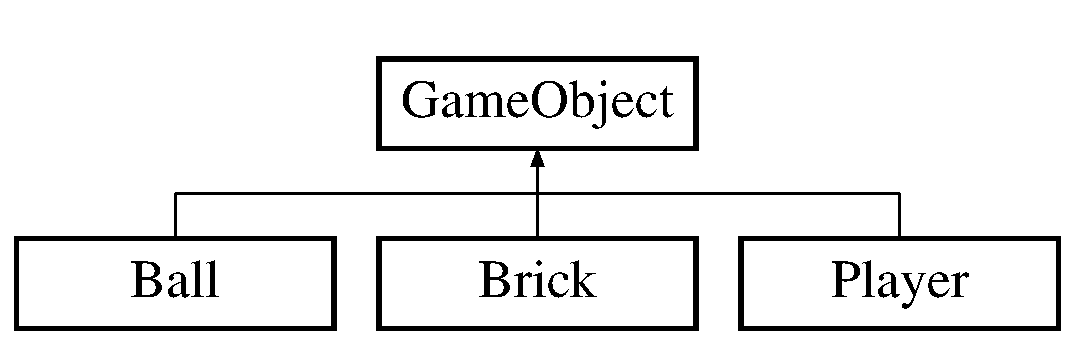
\includegraphics[height=2.000000cm]{class_game_object}
\end{center}
\end{figure}
\subsection*{Public Types}
\begin{DoxyCompactItemize}
\item 
\hypertarget{class_game_object_aa15598edc0e71df4b2765d036cabaf32}{}typedef std\+::vector$<$ std\+::unordered\+\_\+map$<$ int, \hyperlink{class_game_object}{Game\+Object} $\ast$ $>$ $\ast$ $>$ {\bfseries vector\+\_\+of\+\_\+maps\+\_\+gos}\label{class_game_object_aa15598edc0e71df4b2765d036cabaf32}

\item 
\hypertarget{class_game_object_ab21506a575f86173294bd94b3c7a48d3}{}typedef std\+::vector$<$ \hyperlink{class_component}{Component} $\ast$ $>$ {\bfseries vector\+\_\+of\+\_\+components}\label{class_game_object_ab21506a575f86173294bd94b3c7a48d3}

\end{DoxyCompactItemize}
\subsection*{Public Member Functions}
\begin{DoxyCompactItemize}
\item 
\hypertarget{class_game_object_a1fae8627f0de98cedd1457f7253556f3}{}int {\bfseries Get\+Name} () const \label{class_game_object_a1fae8627f0de98cedd1457f7253556f3}

\item 
\hypertarget{class_game_object_a77e945de9f52202defdafeb36d0cca5b}{}S\+D\+L\+\_\+\+Rect $\ast$ {\bfseries Get\+Coords} ()\label{class_game_object_a77e945de9f52202defdafeb36d0cca5b}

\item 
\hypertarget{class_game_object_a4fad55526c42fc5baf1499bc8ab3173c}{}S\+D\+L\+\_\+\+Rect {\bfseries Get\+Coords} () const \label{class_game_object_a4fad55526c42fc5baf1499bc8ab3173c}

\item 
\hypertarget{class_game_object_a411545b4436e623739e5983f2231804f}{}void {\bfseries Add\+Component} (\hyperlink{class_component}{Component} \&component)\label{class_game_object_a411545b4436e623739e5983f2231804f}

\item 
\hypertarget{class_game_object_a1afb5a377cf4f2d8655ca8d5a4e0f088}{}vector\+\_\+of\+\_\+components {\bfseries Get\+Components} () const \label{class_game_object_a1afb5a377cf4f2d8655ca8d5a4e0f088}

\item 
\hypertarget{class_game_object_a6692f17490344d6e95251f9f3d215d2b}{}\hyperlink{class_collision_component}{Collision\+Component} $\ast$ {\bfseries Get\+Collider} () const \label{class_game_object_a6692f17490344d6e95251f9f3d215d2b}

\item 
\hypertarget{class_game_object_ade27cb8f0cd61893efd4c2dee6c0f522}{}void {\bfseries Set\+Collision\+Grid\+Position} (const vector\+\_\+of\+\_\+maps\+\_\+gos \&grid\+\_\+cell)\label{class_game_object_ade27cb8f0cd61893efd4c2dee6c0f522}

\item 
\hypertarget{class_game_object_ab964b02bf537844e8fa159cfa192778d}{}vector\+\_\+of\+\_\+maps\+\_\+gos $\ast$ {\bfseries Get\+Collision\+Grid\+Position} ()\label{class_game_object_ab964b02bf537844e8fa159cfa192778d}

\item 
\hypertarget{class_game_object_af722f1a052cc4933b1dd6c2bf866b0ba}{}vector\+\_\+of\+\_\+maps\+\_\+gos {\bfseries Get\+Collision\+Grid\+Position} () const \label{class_game_object_af722f1a052cc4933b1dd6c2bf866b0ba}

\item 
\hypertarget{class_game_object_a38e4c210f6bb0508ca3868653cd83a06}{}virtual void {\bfseries Handle\+Collision} (const \hyperlink{class_game_object}{Game\+Object} \&)\label{class_game_object_a38e4c210f6bb0508ca3868653cd83a06}

\end{DoxyCompactItemize}
\subsection*{Protected Attributes}
\begin{DoxyCompactItemize}
\item 
\hypertarget{class_game_object_a46fc0e2123b0112a2d1e2d2d4df452cf}{}vector\+\_\+of\+\_\+components {\bfseries components\+\_\+}\label{class_game_object_a46fc0e2123b0112a2d1e2d2d4df452cf}

\end{DoxyCompactItemize}
\subsection*{Friends}
\begin{DoxyCompactItemize}
\item 
\hypertarget{class_game_object_af35fce83d2954152d48746a9f9b2a16d}{}bool {\bfseries operator==} (const \hyperlink{class_game_object}{Game\+Object} \&lhs, const \hyperlink{class_game_object}{Game\+Object} \&rhs)\label{class_game_object_af35fce83d2954152d48746a9f9b2a16d}

\item 
\hypertarget{class_game_object_a0b1778f244697372788e724fee0f776e}{}bool {\bfseries operator!=} (const \hyperlink{class_game_object}{Game\+Object} \&lhs, const \hyperlink{class_game_object}{Game\+Object} \&rhs)\label{class_game_object_a0b1778f244697372788e724fee0f776e}

\end{DoxyCompactItemize}


\subsection{Detailed Description}
This header file declares the base class for all Game\+Objects. 

It is designed to be be subclassed for any objects visible to the player.

\begin{DoxyAuthor}{Author}
Anders Mikkelsen 
\end{DoxyAuthor}
\begin{DoxyVersion}{Version}
1.\+0 
\end{DoxyVersion}
\begin{DoxyDate}{Date}
13.\+04.\+2015 
\end{DoxyDate}


The documentation for this class was generated from the following files\+:\begin{DoxyCompactItemize}
\item 
Game\+Object.\+h\item 
Game\+Object.\+cpp\end{DoxyCompactItemize}

\hypertarget{class_game_object_spawner}{}\section{Game\+Object\+Spawner$<$ T $>$ Class Template Reference}
\label{class_game_object_spawner}\index{Game\+Object\+Spawner$<$ T $>$@{Game\+Object\+Spawner$<$ T $>$}}


This header file declares my generic \hyperlink{class_game_object}{Game\+Object} spawner.  




{\ttfamily \#include $<$Game\+Object\+Spawner.\+h$>$}

\subsection*{Public Member Functions}
\begin{DoxyCompactItemize}
\item 
\hypertarget{class_game_object_spawner_a59b7bb2a3d0805dd286373d2f54df110}{}std\+::shared\+\_\+ptr$<$ T $>$ {\bfseries Spawn} ()\label{class_game_object_spawner_a59b7bb2a3d0805dd286373d2f54df110}

\end{DoxyCompactItemize}


\subsection{Detailed Description}
\subsubsection*{template$<$class T$>$class Game\+Object\+Spawner$<$ T $>$}

This header file declares my generic \hyperlink{class_game_object}{Game\+Object} spawner. 

It is mainly to abstract away the ugly initilization of the object, and to should I know the general idea of how templates are meant to work, although this is an extremely simple template.

\begin{DoxyAuthor}{Author}
Anders Mikkelsen 
\end{DoxyAuthor}
\begin{DoxyVersion}{Version}
1.\+0 
\end{DoxyVersion}
\begin{DoxyDate}{Date}
13.\+04.\+2015 
\end{DoxyDate}


The documentation for this class was generated from the following file\+:\begin{DoxyCompactItemize}
\item 
Game\+Object\+Spawner.\+h\end{DoxyCompactItemize}

\hypertarget{class_input_manager}{}\section{Input\+Manager Class Reference}
\label{class_input_manager}\index{Input\+Manager@{Input\+Manager}}


This header file declares the \hyperlink{class_input_manager}{Input\+Manager}.  




{\ttfamily \#include $<$Input\+Manager.\+h$>$}

\subsection*{Public Member Functions}
\begin{DoxyCompactItemize}
\item 
\hypertarget{class_input_manager_aa5480931dba2720e7d80dd00a53adae0}{}void {\bfseries Update} ()\label{class_input_manager_aa5480931dba2720e7d80dd00a53adae0}

\item 
\hypertarget{class_input_manager_a18ae2fda358d7865fd0f8549cf5e567b}{}void {\bfseries Clear} ()\label{class_input_manager_a18ae2fda358d7865fd0f8549cf5e567b}

\item 
\hypertarget{class_input_manager_a0c2a0e6f88b8c750c2e6a6144c6754cc}{}bool {\bfseries Key\+Down} (int key\+\_\+code)\label{class_input_manager_a0c2a0e6f88b8c750c2e6a6144c6754cc}

\item 
\hypertarget{class_input_manager_ae64fce71b03055787db3b88ceac7a8ae}{}bool {\bfseries Key\+Still\+Down} (int key\+\_\+code)\label{class_input_manager_ae64fce71b03055787db3b88ceac7a8ae}

\item 
\hypertarget{class_input_manager_a5a6d53999798af40b2af8dddfc57db46}{}bool {\bfseries Key\+Up} (int key\+\_\+code)\label{class_input_manager_a5a6d53999798af40b2af8dddfc57db46}

\item 
\hypertarget{class_input_manager_a21c6050d4cf1d7533c42c4719d10921e}{}bool {\bfseries Key\+Still\+Up} (int key\+\_\+code)\label{class_input_manager_a21c6050d4cf1d7533c42c4719d10921e}

\end{DoxyCompactItemize}


\subsection{Detailed Description}
This header file declares the \hyperlink{class_input_manager}{Input\+Manager}. 

It is a trimmed down and slightly optimized version that has been converted to smart pointers.

\begin{DoxyAuthor}{Author}
Anders Mikkelsen 
\end{DoxyAuthor}
\begin{DoxyVersion}{Version}
1.\+0 
\end{DoxyVersion}
\begin{DoxyDate}{Date}
13.\+04.\+2015 
\end{DoxyDate}


The documentation for this class was generated from the following files\+:\begin{DoxyCompactItemize}
\item 
Input\+Manager.\+h\item 
Input\+Manager.\+cpp\end{DoxyCompactItemize}

\hypertarget{class_level_manager}{}\section{Level\+Manager Class Reference}
\label{class_level_manager}\index{Level\+Manager@{Level\+Manager}}


This header file declares the \hyperlink{class_level_manager}{Level\+Manager}.  




{\ttfamily \#include $<$Level\+Manager.\+h$>$}

\subsection*{Public Types}
\begin{DoxyCompactItemize}
\item 
\hypertarget{class_level_manager_aeb43724114a2a794bf3421a8628d4d32}{}typedef std\+::vector$<$ \hyperlink{class_movement_component}{Movement\+Component} $\ast$ $>$ {\bfseries vector\+\_\+of\+\_\+ptrs\+\_\+movement\+\_\+components}\label{class_level_manager_aeb43724114a2a794bf3421a8628d4d32}

\item 
\hypertarget{class_level_manager_aef4b6c259dec0a9db7c4ec9b48011f12}{}typedef std\+::vector$<$ \hyperlink{class_collision_component}{Collision\+Component} $\ast$ $>$ {\bfseries vector\+\_\+of\+\_\+ptrs\+\_\+collision\+\_\+components}\label{class_level_manager_aef4b6c259dec0a9db7c4ec9b48011f12}

\end{DoxyCompactItemize}
\subsection*{Public Member Functions}
\begin{DoxyCompactItemize}
\item 
\hypertarget{class_level_manager_a59a77f39ca9734a471b1464ca86df28b}{}vector\+\_\+of\+\_\+ptrs\+\_\+movement\+\_\+components {\bfseries Get\+Movables} () const \label{class_level_manager_a59a77f39ca9734a471b1464ca86df28b}

\item 
\hypertarget{class_level_manager_a9ba375b7c61050e848e1cccb8e6db26b}{}vector\+\_\+of\+\_\+ptrs\+\_\+collision\+\_\+components {\bfseries Get\+Collidables} () const \label{class_level_manager_a9ba375b7c61050e848e1cccb8e6db26b}

\item 
\hypertarget{class_level_manager_afdd15d07f007a6f7636c600f12a38217}{}void {\bfseries New\+Game} ()\label{class_level_manager_afdd15d07f007a6f7636c600f12a38217}

\item 
\hypertarget{class_level_manager_adfb57eb51fdc979747b72b053b85ad14}{}void {\bfseries Increase\+Level} ()\label{class_level_manager_adfb57eb51fdc979747b72b053b85ad14}

\item 
\hypertarget{class_level_manager_a3a532d8bfb73ebd2d4d730680fc3d6cc}{}\hyperlink{class_player}{Player} $\ast$ {\bfseries Get\+Player} () const \label{class_level_manager_a3a532d8bfb73ebd2d4d730680fc3d6cc}

\item 
\hypertarget{class_level_manager_ab3ed0f936c599c1d69428f97a0240459}{}\hyperlink{class_ball}{Ball} $\ast$ {\bfseries Get\+Ball} () const \label{class_level_manager_ab3ed0f936c599c1d69428f97a0240459}

\item 
\hypertarget{class_level_manager_a5d03144fac306ca2f6d6ece22ff7da64}{}int {\bfseries Get\+Level} () const \label{class_level_manager_a5d03144fac306ca2f6d6ece22ff7da64}

\item 
\hypertarget{class_level_manager_af11dba6a95782f794bf6ce919fd236f2}{}const float \& {\bfseries Get\+Level\+Velocity} () const \label{class_level_manager_af11dba6a95782f794bf6ce919fd236f2}

\item 
\hypertarget{class_level_manager_a7f4c3e316d943742d87622ca3abf59a7}{}int {\bfseries Get\+Player\+Lives} () const \label{class_level_manager_a7f4c3e316d943742d87622ca3abf59a7}

\item 
\hypertarget{class_level_manager_a4dc326928bc59c2c1d14f0efa537e10b}{}void {\bfseries Reduce\+Player\+Lives} ()\label{class_level_manager_a4dc326928bc59c2c1d14f0efa537e10b}

\item 
\hypertarget{class_level_manager_a50df37143640928f6ec730a1d9b59672}{}void {\bfseries Clean\+Up} ()\label{class_level_manager_a50df37143640928f6ec730a1d9b59672}

\end{DoxyCompactItemize}


\subsection{Detailed Description}
This header file declares the \hyperlink{class_level_manager}{Level\+Manager}. 

The \hyperlink{class_level_manager}{Level\+Manager} is responsible for the creation and initialization of all gameplay elements of a level.

In this class i have implemented the Data Locality Pattern for my components, this G\+R\+E\+A\+T\+L\+Y increased the performance of my gameloop.

\begin{DoxyAuthor}{Author}
Anders Mikkelsen 
\end{DoxyAuthor}
\begin{DoxyVersion}{Version}
1.\+0 
\end{DoxyVersion}
\begin{DoxyDate}{Date}
13.\+04.\+2015 
\end{DoxyDate}


The documentation for this class was generated from the following files\+:\begin{DoxyCompactItemize}
\item 
Level\+Manager.\+h\item 
Level\+Manager.\+cpp\end{DoxyCompactItemize}

\hypertarget{class_movement_component}{}\section{Movement\+Component Class Reference}
\label{class_movement_component}\index{Movement\+Component@{Movement\+Component}}
Inheritance diagram for Movement\+Component\+:\begin{figure}[H]
\begin{center}
\leavevmode
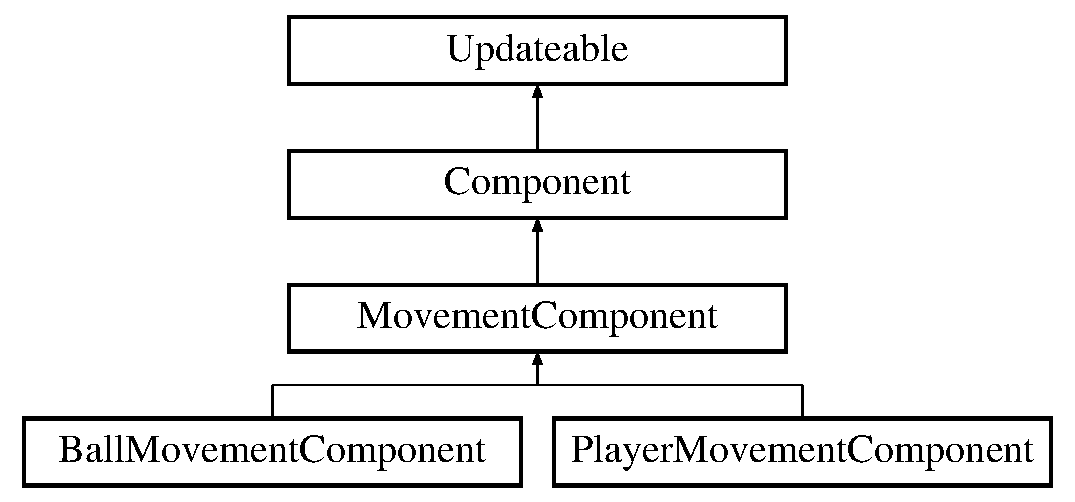
\includegraphics[height=4.000000cm]{class_movement_component}
\end{center}
\end{figure}
\subsection*{Public Member Functions}
\begin{DoxyCompactItemize}
\item 
\hypertarget{class_movement_component_a35279737439b7864d5ecb45e05dbfb51}{}{\bfseries Movement\+Component} (\hyperlink{class_game_object}{Game\+Object} $\ast$const go)\label{class_movement_component_a35279737439b7864d5ecb45e05dbfb51}

\item 
\hypertarget{class_movement_component_a6bb340ec8266ff487d600e36e062943f}{}virtual void {\bfseries Update} () override\label{class_movement_component_a6bb340ec8266ff487d600e36e062943f}

\end{DoxyCompactItemize}
\subsection*{Additional Inherited Members}


The documentation for this class was generated from the following file\+:\begin{DoxyCompactItemize}
\item 
Component.\+h\end{DoxyCompactItemize}

\hypertarget{class_player}{}\section{Player Class Reference}
\label{class_player}\index{Player@{Player}}


This header file declares the \hyperlink{class_player}{Player} subclass of \hyperlink{class_game_object}{Game\+Object}.  




{\ttfamily \#include $<$Player.\+h$>$}

Inheritance diagram for Player\+:\begin{figure}[H]
\begin{center}
\leavevmode
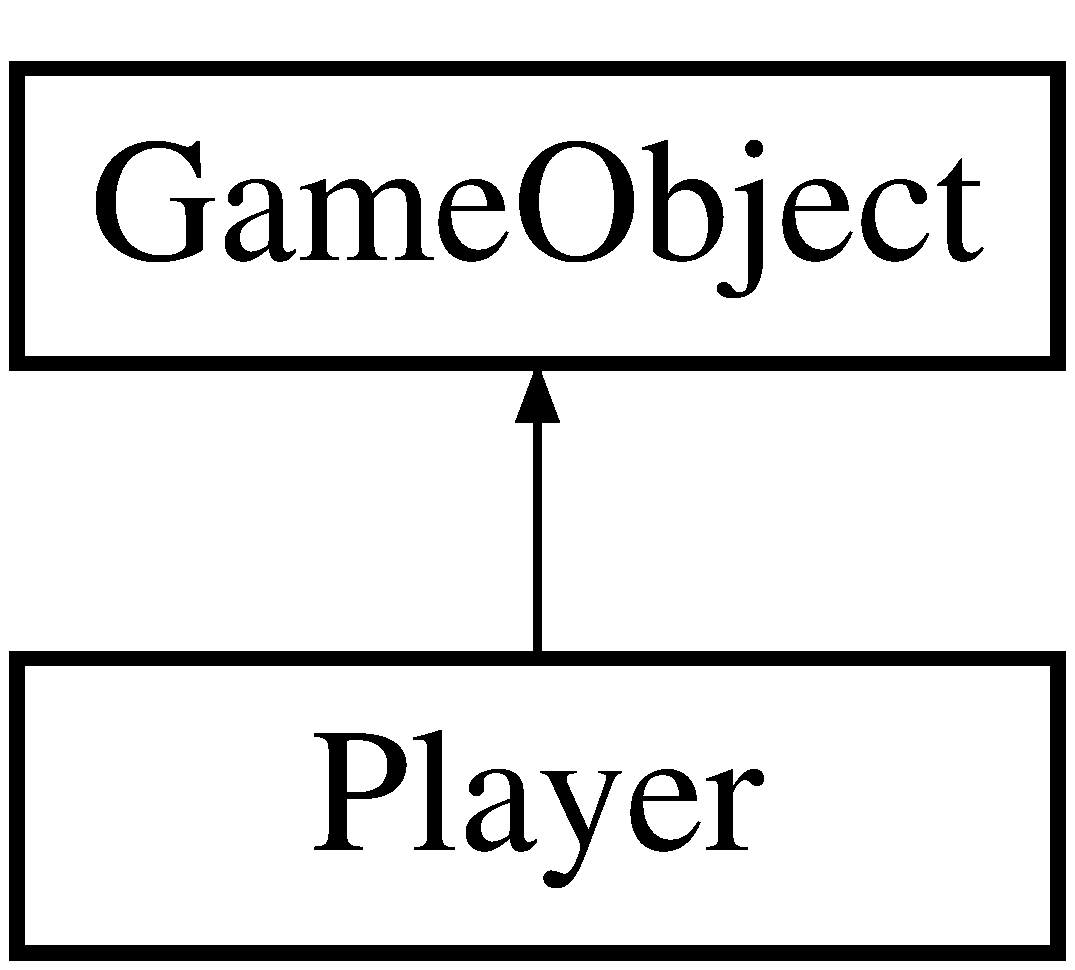
\includegraphics[height=2.000000cm]{class_player}
\end{center}
\end{figure}
\subsection*{Public Member Functions}
\begin{DoxyCompactItemize}
\item 
\hypertarget{class_player_a130256f63476010bc4c42b7eb0a61882}{}S\+D\+L\+\_\+\+Surface $\ast$ {\bfseries Get\+Surface} () const \label{class_player_a130256f63476010bc4c42b7eb0a61882}

\end{DoxyCompactItemize}
\subsection*{Additional Inherited Members}


\subsection{Detailed Description}
This header file declares the \hyperlink{class_player}{Player} subclass of \hyperlink{class_game_object}{Game\+Object}. 

\begin{DoxyAuthor}{Author}
Anders Mikkelsen 
\end{DoxyAuthor}
\begin{DoxyVersion}{Version}
1.\+0 
\end{DoxyVersion}
\begin{DoxyDate}{Date}
13.\+04.\+2015 
\end{DoxyDate}


The documentation for this class was generated from the following files\+:\begin{DoxyCompactItemize}
\item 
Player.\+h\item 
Player.\+cpp\end{DoxyCompactItemize}

\hypertarget{class_player_collision_component}{}\section{Player\+Collision\+Component Class Reference}
\label{class_player_collision_component}\index{Player\+Collision\+Component@{Player\+Collision\+Component}}


This header file declares the component used for handling collisions in the \hyperlink{class_player}{Player} \hyperlink{class_game_object}{Game\+Object}.  




{\ttfamily \#include $<$Player\+Collision\+Component.\+h$>$}

Inheritance diagram for Player\+Collision\+Component\+:\begin{figure}[H]
\begin{center}
\leavevmode
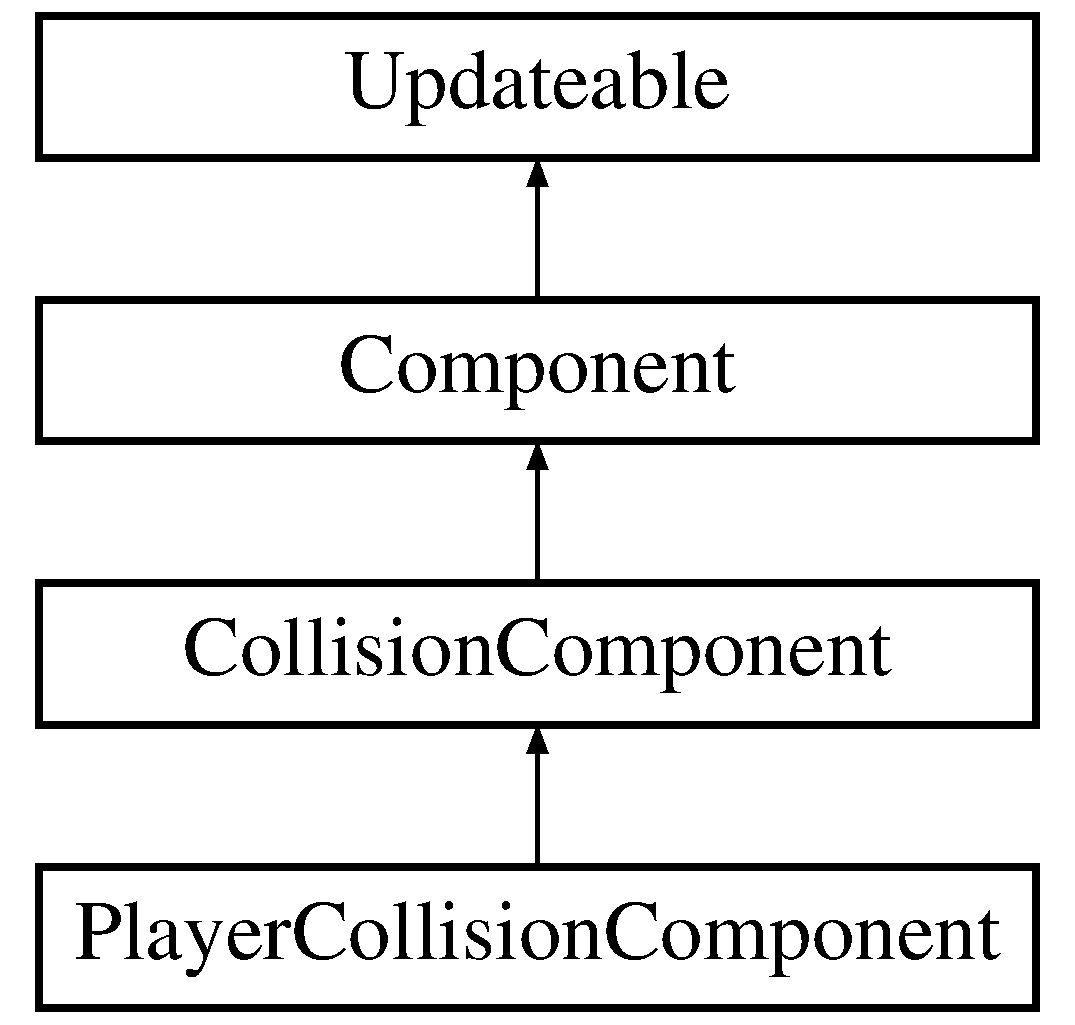
\includegraphics[height=4.000000cm]{class_player_collision_component}
\end{center}
\end{figure}
\subsection*{Public Member Functions}
\begin{DoxyCompactItemize}
\item 
\hypertarget{class_player_collision_component_a007c4a2259a2de566e9fe839d314a85b}{}{\bfseries Player\+Collision\+Component} (\hyperlink{class_game_object}{Game\+Object} $\ast$const go)\label{class_player_collision_component_a007c4a2259a2de566e9fe839d314a85b}

\item 
\hypertarget{class_player_collision_component_a273de888e068ea2968bd60448de19dc0}{}void {\bfseries Update} () override\label{class_player_collision_component_a273de888e068ea2968bd60448de19dc0}

\item 
\hypertarget{class_player_collision_component_a076fe4db176e98dee1d73dc993c747fd}{}void {\bfseries Handle\+Collision} (const \hyperlink{class_game_object}{Game\+Object} \&collidee) override\label{class_player_collision_component_a076fe4db176e98dee1d73dc993c747fd}

\end{DoxyCompactItemize}
\subsection*{Protected Attributes}
\begin{DoxyCompactItemize}
\item 
\hypertarget{class_player_collision_component_aaa64c1874d00d74dae3511cda38fcfb5}{}\hyperlink{class_player}{Player} $\ast$ {\bfseries player\+\_\+}\label{class_player_collision_component_aaa64c1874d00d74dae3511cda38fcfb5}

\end{DoxyCompactItemize}


\subsection{Detailed Description}
This header file declares the component used for handling collisions in the \hyperlink{class_player}{Player} \hyperlink{class_game_object}{Game\+Object}. 

It is updated every frame and is called by Handle\+Collision if involved in a collision.

\begin{DoxyAuthor}{Author}
Anders Mikkelsen 
\end{DoxyAuthor}
\begin{DoxyVersion}{Version}
1.\+0 
\end{DoxyVersion}
\begin{DoxyDate}{Date}
13.\+04.\+2015 
\end{DoxyDate}


The documentation for this class was generated from the following files\+:\begin{DoxyCompactItemize}
\item 
Player\+Collision\+Component.\+h\item 
Player\+Collision\+Component.\+cpp\end{DoxyCompactItemize}

\hypertarget{class_player_movement_component}{}\section{Player\+Movement\+Component Class Reference}
\label{class_player_movement_component}\index{Player\+Movement\+Component@{Player\+Movement\+Component}}


This header file declares the component used for handling movement in the \hyperlink{class_player}{Player} \hyperlink{class_game_object}{Game\+Object}.  




{\ttfamily \#include $<$Player\+Movement\+Component.\+h$>$}

Inheritance diagram for Player\+Movement\+Component\+:\begin{figure}[H]
\begin{center}
\leavevmode
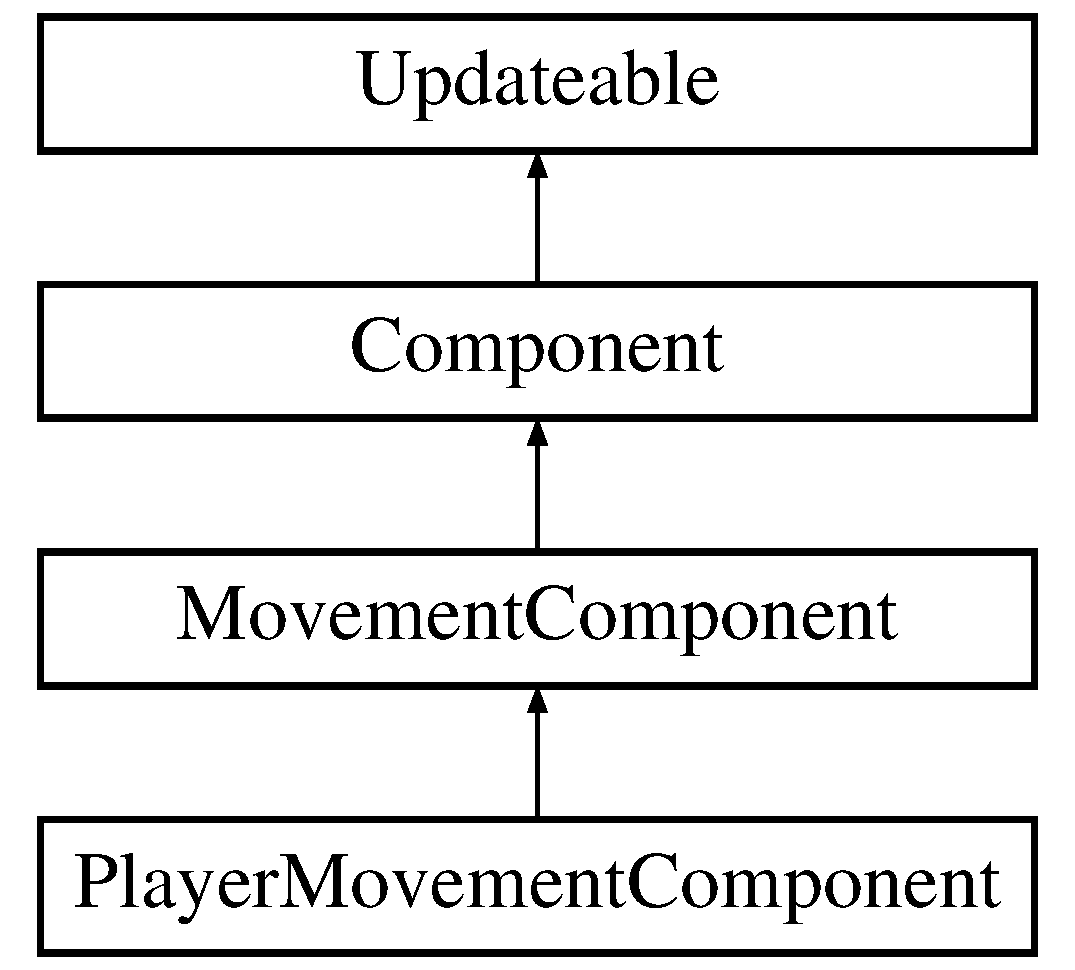
\includegraphics[height=4.000000cm]{class_player_movement_component}
\end{center}
\end{figure}
\subsection*{Public Member Functions}
\begin{DoxyCompactItemize}
\item 
\hypertarget{class_player_movement_component_a447d7b7f468762e0908225bab1ab71fc}{}{\bfseries Player\+Movement\+Component} (\hyperlink{class_game_object}{Game\+Object} $\ast$const go)\label{class_player_movement_component_a447d7b7f468762e0908225bab1ab71fc}

\item 
\hypertarget{class_player_movement_component_a9d70eb70c12cd14116b7bd192e8cfb0b}{}void {\bfseries Update} () override\label{class_player_movement_component_a9d70eb70c12cd14116b7bd192e8cfb0b}

\end{DoxyCompactItemize}
\subsection*{Additional Inherited Members}


\subsection{Detailed Description}
This header file declares the component used for handling movement in the \hyperlink{class_player}{Player} \hyperlink{class_game_object}{Game\+Object}. 

It is updated every frame.

\begin{DoxyAuthor}{Author}
Anders Mikkelsen 
\end{DoxyAuthor}
\begin{DoxyVersion}{Version}
1.\+0 
\end{DoxyVersion}
\begin{DoxyDate}{Date}
13.\+04.\+2015 
\end{DoxyDate}


The documentation for this class was generated from the following files\+:\begin{DoxyCompactItemize}
\item 
Player\+Movement\+Component.\+h\item 
Player\+Movement\+Component.\+cpp\end{DoxyCompactItemize}

\hypertarget{class_score_manager}{}\section{Score\+Manager Class Reference}
\label{class_score_manager}\index{Score\+Manager@{Score\+Manager}}


This header file declares the \hyperlink{class_score_manager}{Score\+Manager}.  




{\ttfamily \#include $<$Score\+Manager.\+h$>$}

\subsection*{Public Types}
\begin{DoxyCompactItemize}
\item 
\hypertarget{class_score_manager_a98638d13e649616b30abf546bb9cca28}{}typedef std\+::vector$<$ std\+::string $>$ {\bfseries vector\+\_\+of\+\_\+strings}\label{class_score_manager_a98638d13e649616b30abf546bb9cca28}

\end{DoxyCompactItemize}
\subsection*{Public Member Functions}
\begin{DoxyCompactItemize}
\item 
\hypertarget{class_score_manager_aa8258601779b7261a5329f31b8a90289}{}int {\bfseries Get\+Score} ()\label{class_score_manager_aa8258601779b7261a5329f31b8a90289}

\item 
\hypertarget{class_score_manager_a36e3e78df80f0741cfb6545ab4ee04ef}{}void {\bfseries Add\+Score} (const \hyperlink{class_game_object}{Game\+Object} \&go, int current\+\_\+level)\label{class_score_manager_a36e3e78df80f0741cfb6545ab4ee04ef}

\item 
\hypertarget{class_score_manager_af4a600e8ec22bdbb5bf62d8c2fae2601}{}void {\bfseries Reset} ()\label{class_score_manager_af4a600e8ec22bdbb5bf62d8c2fae2601}

\item 
\hypertarget{class_score_manager_acb62eef0bc732ae6fa1d5d12147bd594}{}vector\+\_\+of\+\_\+strings {\bfseries Get\+High\+Scores} () const \label{class_score_manager_acb62eef0bc732ae6fa1d5d12147bd594}

\item 
\hypertarget{class_score_manager_ad0e31645100ecb55815c4af56ef79abe}{}void {\bfseries Write\+High\+Scores} (const std\+::vector$<$ std\+::string $>$ \&results)\label{class_score_manager_ad0e31645100ecb55815c4af56ef79abe}

\end{DoxyCompactItemize}
\subsection*{Static Public Attributes}
\begin{DoxyCompactItemize}
\item 
\hypertarget{class_score_manager_aa99fd79728463ba32eaccb54de34c1ac}{}static const int {\bfseries H\+I\+G\+H\+\_\+\+S\+C\+O\+R\+E\+\_\+\+L\+I\+M\+I\+T} = 5\label{class_score_manager_aa99fd79728463ba32eaccb54de34c1ac}

\end{DoxyCompactItemize}


\subsection{Detailed Description}
This header file declares the \hyperlink{class_score_manager}{Score\+Manager}. 

The \hyperlink{class_score_manager}{Score\+Manager} is responsible for keeping track of the current score and creating and writing a resultlist to/from file.

\begin{DoxyAuthor}{Author}
Anders Mikkelsen 
\end{DoxyAuthor}
\begin{DoxyVersion}{Version}
1.\+0 
\end{DoxyVersion}
\begin{DoxyDate}{Date}
13.\+04.\+2015 
\end{DoxyDate}


The documentation for this class was generated from the following files\+:\begin{DoxyCompactItemize}
\item 
Score\+Manager.\+h\item 
Score\+Manager.\+cpp\end{DoxyCompactItemize}

\hypertarget{class_s_d_l_initialization_exception}{}\section{S\+D\+L\+Initialization\+Exception Class Reference}
\label{class_s_d_l_initialization_exception}\index{S\+D\+L\+Initialization\+Exception@{S\+D\+L\+Initialization\+Exception}}


This header file declares the Exception class i made for showing that i understand how they work.  




{\ttfamily \#include $<$S\+D\+L\+Initialization\+Exception.\+h$>$}

Inheritance diagram for S\+D\+L\+Initialization\+Exception\+:\begin{figure}[H]
\begin{center}
\leavevmode
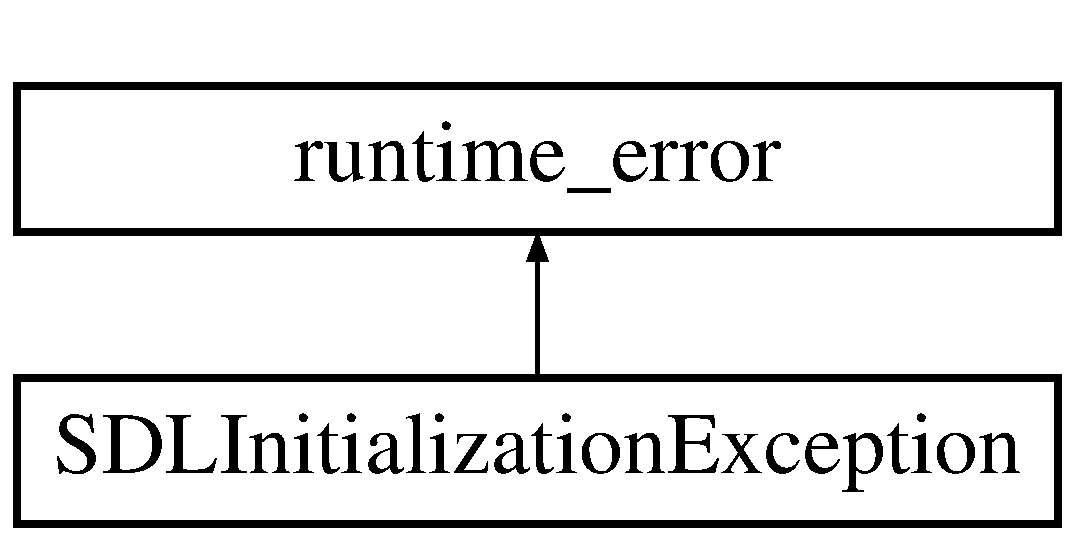
\includegraphics[height=2.000000cm]{class_s_d_l_initialization_exception}
\end{center}
\end{figure}


\subsection{Detailed Description}
This header file declares the Exception class i made for showing that i understand how they work. 

I have restricted its use for initialization so it will not impact performance in any way.

\begin{DoxyAuthor}{Author}
Anders Mikkelsen 
\end{DoxyAuthor}
\begin{DoxyVersion}{Version}
1.\+0 
\end{DoxyVersion}
\begin{DoxyDate}{Date}
13.\+04.\+2015 
\end{DoxyDate}


The documentation for this class was generated from the following files\+:\begin{DoxyCompactItemize}
\item 
S\+D\+L\+Initialization\+Exception.\+h\item 
S\+D\+L\+Initialization\+Exception.\+cpp\end{DoxyCompactItemize}

\hypertarget{class_s_d_lsound}{}\section{S\+D\+Lsound Class Reference}
\label{class_s_d_lsound}\index{S\+D\+Lsound@{S\+D\+Lsound}}


This header file declares the facade for S\+D\+L\+\_\+mixer.  




{\ttfamily \#include $<$S\+D\+Lsound.\+h$>$}

\subsection*{Public Types}
\begin{DoxyCompactItemize}
\item 
\hypertarget{class_s_d_lsound_a27bf722536cbdd17222b44edbbec4e49}{}enum {\bfseries E\+Song} \{ {\bfseries I\+N\+T\+R\+O\+\_\+\+M\+U\+S\+I\+C}, 
{\bfseries G\+A\+M\+E\+\_\+\+M\+U\+S\+I\+C}, 
{\bfseries G\+A\+M\+E\+O\+V\+E\+R\+\_\+\+M\+U\+S\+I\+C}
 \}\label{class_s_d_lsound_a27bf722536cbdd17222b44edbbec4e49}

\item 
\hypertarget{class_s_d_lsound_ab679a879ea206f956c579f785a3973cc}{}enum {\bfseries E\+Sound} \{ {\bfseries P\+L\+A\+Y\+E\+R\+\_\+\+H\+I\+T\+\_\+\+S\+O\+U\+N\+D}, 
{\bfseries B\+R\+I\+C\+K\+\_\+\+H\+I\+T\+\_\+\+S\+O\+U\+N\+D}, 
{\bfseries B\+A\+L\+L\+\_\+\+D\+E\+A\+T\+H\+\_\+\+S\+O\+U\+N\+D}
 \}\label{class_s_d_lsound_ab679a879ea206f956c579f785a3973cc}

\end{DoxyCompactItemize}
\subsection*{Public Member Functions}
\begin{DoxyCompactItemize}
\item 
\hypertarget{class_s_d_lsound_a407dc7704779a2bd25895d0f70aaba75}{}void {\bfseries Init} ()\label{class_s_d_lsound_a407dc7704779a2bd25895d0f70aaba75}

\item 
\hypertarget{class_s_d_lsound_a2cbfa4bc2f720c1d7f6782796373582d}{}void {\bfseries Kill} ()\label{class_s_d_lsound_a2cbfa4bc2f720c1d7f6782796373582d}

\item 
\hypertarget{class_s_d_lsound_aa25c6a8e6653fbf92d61577e0367948a}{}bool {\bfseries Is\+Music\+Playing} ()\label{class_s_d_lsound_aa25c6a8e6653fbf92d61577e0367948a}

\item 
\hypertarget{class_s_d_lsound_ad1f30c7cdbcec3ce8e33bb3a8719cbcf}{}void {\bfseries Play\+Song} (E\+Song song)\label{class_s_d_lsound_ad1f30c7cdbcec3ce8e33bb3a8719cbcf}

\item 
\hypertarget{class_s_d_lsound_a29af593912b3be92b465726cabc75a5c}{}void {\bfseries Swap\+Song} (E\+Song song)\label{class_s_d_lsound_a29af593912b3be92b465726cabc75a5c}

\item 
\hypertarget{class_s_d_lsound_a7545264d62aecd3ccda80de15a7879e8}{}void {\bfseries Kill\+Song} ()\label{class_s_d_lsound_a7545264d62aecd3ccda80de15a7879e8}

\item 
\hypertarget{class_s_d_lsound_a623308fa01a7d506d196966b22bea59d}{}void {\bfseries Play\+Sound} (E\+Sound sound)\label{class_s_d_lsound_a623308fa01a7d506d196966b22bea59d}

\end{DoxyCompactItemize}


\subsection{Detailed Description}
This header file declares the facade for S\+D\+L\+\_\+mixer. 

In this class I declare all consts for songs and sound have provided a simple enum interface for playing songs and sounds.

\begin{DoxyAuthor}{Author}
Anders Mikkelsen 
\end{DoxyAuthor}
\begin{DoxyVersion}{Version}
1.\+0 
\end{DoxyVersion}
\begin{DoxyDate}{Date}
13.\+04.\+2015 
\end{DoxyDate}


The documentation for this class was generated from the following files\+:\begin{DoxyCompactItemize}
\item 
S\+D\+Lsound.\+h\item 
S\+D\+Lsound.\+cpp\end{DoxyCompactItemize}

\hypertarget{class_s_d_lvideo}{}\section{S\+D\+Lvideo Class Reference}
\label{class_s_d_lvideo}\index{S\+D\+Lvideo@{S\+D\+Lvideo}}


This header file declares the facade for S\+D\+L video rendering.  




{\ttfamily \#include $<$S\+D\+Lvideo.\+h$>$}

\subsection*{Public Types}
\begin{DoxyCompactItemize}
\item 
\hypertarget{class_s_d_lvideo_a6c44bc386fc88f9576e6fc3c14048aa7}{}typedef std\+::vector$<$ std\+::shared\+\_\+ptr$<$ \hyperlink{class_game_object}{Game\+Object} $>$ $>$ {\bfseries vector\+\_\+of\+\_\+shared\+\_\+ptr\+\_\+gos}\label{class_s_d_lvideo_a6c44bc386fc88f9576e6fc3c14048aa7}

\item 
\hypertarget{class_s_d_lvideo_ab8cfa7af7d08ef2e9e6d040c8504eb2f}{}typedef std\+::vector$<$ std\+::string $>$ {\bfseries vector\+\_\+of\+\_\+strings}\label{class_s_d_lvideo_ab8cfa7af7d08ef2e9e6d040c8504eb2f}

\end{DoxyCompactItemize}
\subsection*{Public Member Functions}
\begin{DoxyCompactItemize}
\item 
\hypertarget{class_s_d_lvideo_aaf4d2054fa5a4a05a37d3f1c0cc3b728}{}void {\bfseries Init} ()\label{class_s_d_lvideo_aaf4d2054fa5a4a05a37d3f1c0cc3b728}

\item 
\hypertarget{class_s_d_lvideo_ab15173dc06278a380a59e512020cb40c}{}void {\bfseries Clean\+Up} ()\label{class_s_d_lvideo_ab15173dc06278a380a59e512020cb40c}

\item 
\hypertarget{class_s_d_lvideo_a5f6045e76aeac461a424597ac4905183}{}bool {\bfseries Kill} ()\label{class_s_d_lvideo_a5f6045e76aeac461a424597ac4905183}

\item 
\hypertarget{class_s_d_lvideo_ab8588460623d611ef25951514eaf1729}{}void {\bfseries Update} (E\+Game\+State game\+\_\+state, const vector\+\_\+of\+\_\+shared\+\_\+ptr\+\_\+gos \&game\+\_\+objects, int level, int current\+\_\+lives, int current\+\_\+score)\label{class_s_d_lvideo_ab8588460623d611ef25951514eaf1729}

\item 
\hypertarget{class_s_d_lvideo_ad10a8ab09774fb1771029e60146ed794}{}void {\bfseries Create\+Intro\+Texture} ()\label{class_s_d_lvideo_ad10a8ab09774fb1771029e60146ed794}

\item 
\hypertarget{class_s_d_lvideo_a06674910d743bb041e69f8cb40440f8c}{}void {\bfseries Create\+Game\+Over\+Texture} (bool new\+\_\+high\+\_\+score, vector\+\_\+of\+\_\+strings results)\label{class_s_d_lvideo_a06674910d743bb041e69f8cb40440f8c}

\item 
\hypertarget{class_s_d_lvideo_aa7004dc8ba964525a7725682e7ee1621}{}void {\bfseries Create\+Player\+Texture} (const \hyperlink{class_player}{Player} \&player)\label{class_s_d_lvideo_aa7004dc8ba964525a7725682e7ee1621}

\item 
\hypertarget{class_s_d_lvideo_a592243f65a44b39361367228161c273e}{}void {\bfseries Create\+Brick\+Texture} (const \hyperlink{class_brick}{Brick} \&brick)\label{class_s_d_lvideo_a592243f65a44b39361367228161c273e}

\item 
\hypertarget{class_s_d_lvideo_ad0b3b6623069a38ab9ec7250527139a4}{}void {\bfseries Create\+Ball\+Texture} (const \hyperlink{class_ball}{Ball} \&ball)\label{class_s_d_lvideo_ad0b3b6623069a38ab9ec7250527139a4}

\item 
\hypertarget{class_s_d_lvideo_aaaa0f579f5035b50218be9e52fc778b3}{}void {\bfseries Kill\+Game\+Object\+Texture} (const \hyperlink{class_game_object}{Game\+Object} \&go)\label{class_s_d_lvideo_aaaa0f579f5035b50218be9e52fc778b3}

\end{DoxyCompactItemize}
\subsection*{Static Public Member Functions}
\begin{DoxyCompactItemize}
\item 
\hypertarget{class_s_d_lvideo_a15a3bde646d6744fbb97a49b50761454}{}static int {\bfseries Get\+Screen\+Width} ()\label{class_s_d_lvideo_a15a3bde646d6744fbb97a49b50761454}

\item 
\hypertarget{class_s_d_lvideo_a267b3503399bc79c2fa2cbaff30d1361}{}static int {\bfseries Get\+Screen\+Height} ()\label{class_s_d_lvideo_a267b3503399bc79c2fa2cbaff30d1361}

\item 
\hypertarget{class_s_d_lvideo_a8a1d40aea3d2cf50e865a3413f6ea793}{}static int {\bfseries Get\+G\+U\+I\+Area} ()\label{class_s_d_lvideo_a8a1d40aea3d2cf50e865a3413f6ea793}

\end{DoxyCompactItemize}


\subsection{Detailed Description}
This header file declares the facade for S\+D\+L video rendering. 

It accepts normal game mechanical items such as Game\+Objects and gui texts and abstracts away any S\+D\+L for the outside classes.

I showcase use of S\+D\+L\+\_\+image for pngs for the player and ball, normal B\+M\+P for bricks.

\begin{DoxyAuthor}{Author}
Anders Mikkelsen 
\end{DoxyAuthor}
\begin{DoxyVersion}{Version}
1.\+0 
\end{DoxyVersion}
\begin{DoxyDate}{Date}
13.\+04.\+2015 
\end{DoxyDate}


The documentation for this class was generated from the following files\+:\begin{DoxyCompactItemize}
\item 
S\+D\+Lvideo.\+h\item 
S\+D\+Lvideo.\+cpp\end{DoxyCompactItemize}

\hypertarget{class_updateable}{}\section{Updateable Class Reference}
\label{class_updateable}\index{Updateable@{Updateable}}


This header file declares the different abstract and concrete interfaces I use for components.  




{\ttfamily \#include $<$Component.\+h$>$}

Inheritance diagram for Updateable\+:\begin{figure}[H]
\begin{center}
\leavevmode
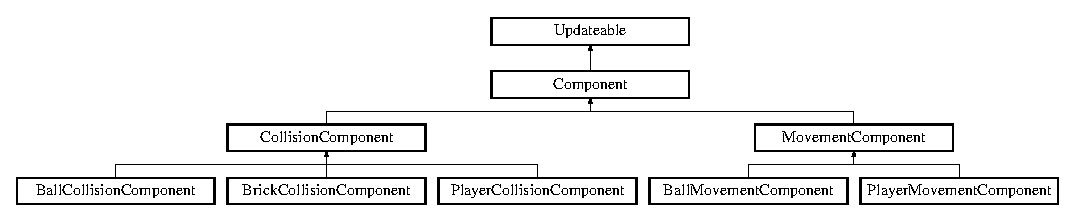
\includegraphics[height=2.516854cm]{class_updateable}
\end{center}
\end{figure}
\subsection*{Public Member Functions}
\begin{DoxyCompactItemize}
\item 
\hypertarget{class_updateable_a162a673ad3268dcfc9dd382e35122ebe}{}virtual void {\bfseries Update} ()=0\label{class_updateable_a162a673ad3268dcfc9dd382e35122ebe}

\end{DoxyCompactItemize}


\subsection{Detailed Description}
This header file declares the different abstract and concrete interfaces I use for components. 

\begin{DoxyAuthor}{Author}
Anders Mikkelsen 
\end{DoxyAuthor}
\begin{DoxyVersion}{Version}
1.\+0 
\end{DoxyVersion}
\begin{DoxyDate}{Date}
13.\+04.\+2015 
\end{DoxyDate}


The documentation for this class was generated from the following file\+:\begin{DoxyCompactItemize}
\item 
Component.\+h\end{DoxyCompactItemize}

%--- End generated contents ---

% Index
\backmatter
\newpage
\phantomsection
\clearemptydoublepage
\addcontentsline{toc}{chapter}{Index}
\printindex

\end{document}
